\documentclass{article}


\usepackage[nottoc]{tocbibind}
\usepackage[backend=biber]{biblatex}
\bibliography{References.bib}


\usepackage{amsmath}
\usepackage{cleveref}
\usepackage{mathtools}
\usepackage{amsfonts}
\usepackage{amssymb}
\usepackage{standalone}
\usepackage{multirow}
\usepackage{subfigure}
\usepackage{graphicx}
\usepackage{caption}
\usepackage{bm}
\usepackage{gensymb}
\usepackage{siunitx}
\usepackage{float}
\usepackage{tikz}
\usepackage{tikz-3dplot}
\usetikzlibrary{calc}

\newcommand{\me}{\mathrm{e}}
\providecommand{\abs}[1]{\lvert#1\rvert} \providecommand{\norm}[1]{\lVert#1\rVert}

\makeatletter
\newsavebox{\@brx}
\newcommand{\llangle}[1][]{\savebox{\@brx}{\(\m@th{#1\langle}\)}%
	\mathopen{\copy\@brx\mkern2mu\kern-0.9\wd\@brx\usebox{\@brx}}}
\newcommand{\rrangle}[1][]{\savebox{\@brx}{\(\m@th{#1\rangle}\)}%
	\mathclose{\copy\@brx\mkern2mu\kern-0.9\wd\@brx\usebox{\@brx}}}
\makeatother

\numberwithin{equation}{section}

\title{Licenciate}
\author{Kajsa-My Blomdahl}
\date{October 2018}
\begin{document}

\maketitle

\tableofcontents

\section{Background}
\subsection{The Three-body Problem}
The $n$-body problem is a class of problems in physics that, in a highly general sense, consists of modelling the motion of $n$ objects interacting through some physical force. In classical mechanics the equations of motion for $n$ point particles can be derived from Newton's second law of motion, which states that the rate of change in momentum for an object equals the force acting on it, or from analytical formulations such as Lagrangian and Hamiltonian mechanics, which consider scalar properties of motion like kinetic and potential energies. In the quantum regime, where the wave-like property of matter has to be taken into account, the state of an $n$-body system is described by a total wave function, where the Hamiltonian operator generates the time evolution of the state as given by Schr{\"o}dinger's differential equation.

The core of the $n$-body problem is that neither the classical equations of motion nor the Schr{\"o}dinger equation are analytically solvable for more than two interacting particles. Consider the case where $n=3$. Although apparently simple, the configuration space for the three-body problem is six dimensional after separating out the center of mass motion. Three additional constants of motion can be provided by conservation of the total angular momentum, which effectively reduces the problem to that of three coupled second order non-linear differential equations in the classical case and a three dimensional Schr{\"o}dinger equation in the quantum case. 

The quest for a general solution to the classical three-body problem is renowned. As a recurrent muse to a number of great mathematicians during the past centuries, dating back to Newton himself, the three-body problem has been a catalyst for the development of analysis and the modern theory of dynamical systems \cite{Chenciner2015}. Although there are a number of special cases that have explicit solutions, non-linear dynamical systems often display highly unpredictable behaviour due to sensitive dependencies on initial conditions, i.e. are chaotic. Nowadays, different numerical approaches are used to solve these kinds of problems, but the computational load can be substantial. 

In contrast to the classical case, the quantum three-body problem is amenable to qualitative analysis \cite{efimov1990qualitative} and in some cases, even to analytic solutions. In the quantum realm of few-body systems the Faddeev and the Faddeev-Yakubovsky equations, which are equivalent formulations of the Schr{\"o}dinger equation for three- and four-body systems respectively, can, for a few special cases, be solved analytically by iteration \cite{Faddeev:1960su, Zubarev:1994}. For the three-body scattering problem bound state solutions can exist in cases where all three two-body subsystems have short-ranged interactions, if at least two of these interactions are close to resonance. This is called the Efimov effect. 

\subsection{The Birth of Efimov Physics}
In low energy scattering, particles are said to resonate when the strength of the attractive interaction between them barely cancels out the repulsive effect of the kinetic energy. During the collision they remain close for an extended period of time, in an almost bound state, before separating. 

In 1970, Vitaly Efimov predicted that resonant two-body forces could give rise to a series of bound energy levels in three-particle systems \cite{Efimov:1970zz}. When the short-ranged two-body forces approached resonance, he found a universal long-range three-body attraction emerging, giving rise to an infinite number of trimer states with binding energies obeying a discrete scaling law at resonance.  
 
Efimov proposed that attractive three-body interaction appearing in systems with resonant short-ranged interactions and repulsive Coulomb forces could explain the binding of three particle nuclei such as the three nucleon triton $\prescript{3}{}{\mathrm{H}}$ and the triple-alpha Hoyle state of $\prescript{12}{}{\mathrm{C}}$.

The notion of Efimov physics comprises a range of universal phenomena that occur in few-body systems exhibiting the Efimov effect. Short-ranged forces commonly occur in nature and few-body effects are expected to appear in a broad range of physical systems. Development in the theory of few-body quantum systems is important since it could bridge the gap between existing well developed models of treating one- and two-body systems and the statistical methods used to describe many-body systems.

\section{Introduction} 
\subsection{Scattering Theory}
A short reveiw concerning some important aspects of quantum mechanical systems and two-body scattering, in particlular the concept of \emph{scattering length}, will follow in order to set the stage for a discussion of quantum effects in few-body systems in general and Efimov states in three-body systems in particular. 

\subsubsection{Entering the quantum realm}
All particles of matter exhibit wave-like properties. The wavelength of a particle with momentum $p$ is given by the de Broglie equation

\begin{equation} \label{eq:1}
\lambda = \frac{h}{p} = \frac{h}{mv}
\end{equation}
where $h$ is the Planck constant. The wave characteristics of matter grow with increasing de Broglie wavelength. When the wavelength is sufficently large, classical physics no longer applies and the system has reached the quantum regime. From \ref{eq:1} it is evident that this is true for particles that are very small or very slow. In an ultracold quantum gas, the atoms are cooled down to a point where they move so slowly that the increased uncertainty in position for the individual atoms becomes so large that they start to overlap with eachother. At this point the atoms cannot be viewed as individual particles but as a correlated wave. The de Broglie wavelength of the atoms is then larger than the average interatomic spacing, which is about one micron in a low density gas, and their behaviour are fully governed by quantum mechanics. In other words, the transition to the quantum regime occures when the thermal de Broglie wavelength is on the order of the interparticle spacing. Since the temperature of the gas and the thermal de Broglie wavelength are related through

\begin{equation}
\lambda = \frac{h}{\sqrt{2\pi m k_B T}},
\end{equation}
in which $k_B$ is the Boltzmann constant, it means there is a critical temperature for when the quantum effects becomes dominant. For a dilute atomic gas this critical temperature are in the microkelvin to nanokelvin range.
 
\subsubsection{Two-body Scattering} \label{Two-body scattering}
A collision between a pair of particles can be described in their center-of-mass frame as the scattering of a particle with reduced mass $\mu$ ($\mu = m_1m_2/(m_1 + m_2)$) by the potential $V(\mathbf{r})$. The time-independent  Schr{\"o}dinger equation for the relative motion is then given by 

\begin{equation} \label{eq:22}
\bigg[-\frac{\hbar^2}{2\mu}\nabla^2 + V(\mathbf{r})\bigg]\psi(\mathbf{r}) = \frac{\hbar^2 k^2}{2 \mu}\psi(\mathbf{r}),
\end{equation}
where $\mathbf{r}$ denotes the interparticle separation, $k$ is the wave number ($k=p/\hbar = \sqrt{2\mu E}/\hbar$) and $\nabla^2$ the Laplace operator, which in spherical coordinates reads

\begin{equation} \label{eq:23}
\nabla^2 = \frac{1}{r^2} \frac{\partial}{\partial r} \bigg(r^2 \frac{\partial}{\partial r}\bigg) + \frac{1}{r^2 \sin\theta} \frac{\partial}{\partial\theta} \bigg(\sin\theta \frac{\partial}{\partial\theta}\bigg) + \frac{1}{r^2 \sin^2\theta} \frac{\partial^2}{\partial\phi^2}.
\end{equation}
By requiring the potential to be zero at large interparticle separation, the collision can be described as that of an incident plane wave with definite angular momentum that scatters off a potential placed at the origin. The potential will deflect some of the incident waves to form scattered waves, which at large distances will be diverging from a point source in the scattering region. Let $r_0$ denote the range of the action of the potential and let $z$ denote the direction of the propagation of the incident plane wave. The boundary condition at large separations $r \gg r_0$ then imposes a solution of the following asymptotic form

\begin{equation}\label{eq:26}
\psi(\mathbf{r}) \xrightarrow{r \to \infty} e^{ikz} + f(k,\theta,\phi)\frac{e^{ikr}}{r},
\end{equation}
in which the total wave function is written as a superposition of the incident and scattered wave, with a scattering amplitude $f(k,\theta,\phi)$ that depends on the energy of the particle through $k$, the deflection angle $\theta$ between the waves and the azimuthal angle $\phi$ about the $z$-axis. For spherically symmetric potentials, i.e. $V(\mathbf{r}) = V(r)$, the Schr{\"o}dinger equation \eqref{eq:22} is separable. The incident and scattered wave functions are then conveniently expanded on a basis set of eigenfunctions of $\mathbf{L}^2$ and $L_z$, where $\mathbf{L}$ is the relative orbital angular momentum operator. These eigenfunctions are the spherical harmonic functions $Y_l^m(\theta,\phi)$, which satisfy 

\begin{equation}
\mathbf{L}^2 Y_l^m(\theta,\phi) \equiv -\frac{1}{ \sin^2\theta} \bigg[ \sin\theta \frac{\partial}{\partial\theta} \bigg(\sin\theta \frac{\partial}{\partial\theta}\bigg) +  \frac{\partial^2}{\partial\phi^2}\bigg] Y_l^m(\theta,\phi) = l(l+1)Y_l^m(\theta,\phi).
\end{equation}
The most general solution to \eqref{eq:22} is then of the form

\begin{equation}\label{eq:32}
\psi(\mathbf{r}) = \sum_{l=0}^{\infty} \sum_{m = -l}^{l} C_{lm}\frac{u_{l}(r)}{r}Y_l^m(\theta,\phi).
\end{equation}
The separability of $\psi(\mathbf{r})$ effectively reduces the problem to that of solving the radial equation

\begin{equation} \label{eq:24}
\bigg[-\frac{d^2}{dr^2} + \frac{l(l+1)}{r^2} + \frac{2\mu}{\hbar^2}V(r) - k^2\bigg]u_l(r) = 0.
\end{equation}
By requiring the wave function to be finite  everywhere it is implied that $u_l(r)$ must vanish at the origin. In the case where $V(r) = 0$, the solutions to the radial equation for positive energies have the form

\begin{equation}
u_l(r) \sim r j_l(kr),
\end{equation}
where $j_l(kr)$ are the spherical Bessel functions. In the case of a non-zero potential the solutions needs to be regular at the origin, while at large distances $r \gg r_0$ they have the form

\begin{equation}\label{eq:25}
u_l(r) = r(a_l j_l(kr)+b_l y_l(kr)),
\end{equation} 
where $y_l(kr)$ are the spherical Neumann functions. Asymptotically the solutions \eqref{eq:25} behave like

\begin{equation}
u_l(r) \xrightarrow{r\to\infty} \frac{1}{k}\big(a_l \sin(kr - l\frac{\pi}{2})-b_l \cos(kr - l\frac{\pi}{2})\big).
\end{equation} 
By defining the ratio of the coefficients as

\begin{equation}
\frac{b_l}{a_l} = -\tan\delta_l(k),
\end{equation} 
where $\delta_l(k)$ is an energy dependent phase shift, the normalized asymptotic radial solutions for a non-vanishing potential can be written

\begin{equation}
\begin{split}
u_l(r) \xrightarrow{r \to \infty} &\frac{1}{k}\big(\sin(kr - l\frac{\pi}{2} + \delta_l(k))\big)\\
=&\frac{e^{-i\delta_l{k}}}{2ik}\big((-1)^{l+1}e^{-ikr} + e^{2i\delta_l(k)e^{ikr}}\big).
\end{split}
\end{equation}
Since the incident plane wave \eqref{eq:26} is aligned with the $z$-axis, it is an eigenfunction of $L_z$ with eigenvalue $m=0$. The plane wave expansion is thus independent of the azimuthal angle around the $z$-axis and can therefore be expressed as

\begin{equation}\label{eq:27}
e^{ikz} = \sum_{l=0}^{\infty} (2l+1)i^l j_l(kr)P_l(\cos\theta),
\end{equation}
where $P_l(\cos\theta)$ are Legendre polynomials. It is evident that this plane wave is a solution to \eqref{eq:22} for $V(r) = 0$. Asymptotically the solutions \eqref{eq:27} behave like

\begin{equation}\label{eq:29}
e^{ikz} \xrightarrow{r \to \infty} \frac{1}{2ikr} \sum_{l=0}^{\infty} (2l+1)P_l(\cos\theta)\big((-1)^{l+1}e^{-ikr} + e^{ikr}\big).
\end{equation}
The incident plane wave can thus be resolved into that of incoming ($e^{-ikr}$) and outgoing ($e^{ikr}$) spherical waves with a relative phase of $0$ for $l$ with odd parity and $\pi$ otherwise. The scattering amplitude is Substituting \eqref{eq:29} into \eqref{eq:26} results in an asymptotic wave function of the form

\begin{equation}\label{eq:30}
\psi(\mathbf{r}) \xrightarrow{r \to \infty} \frac{1}{2ikr}\sum_{l=0}^{\infty} (2l+1)P_l(\cos\theta))\big((-1)^{l+1}e^{-ikr} + e^{ikr}\big) + f(k, \theta) \frac{e^{ikr}}{r},
\end{equation} 
where $f(k,\theta,\phi)=f(k,\theta)$ because the scattering potential is spherically symmetric. Since the system is rotationally invariant about the $z$-axis, the scattered wave function must be azimuthally symmetric, i.e. have magnetic quantum number $m=0$, wherefore the general solution \eqref{eq:32} becomes

\begin{equation}\label{eq:28}
\psi(\mathbf{r}) = \sum_{l=0}^{\infty} c_l \frac{u_l(r)}{r} P_l(\cos\theta),
\end{equation} 
in which $c_l$ are unknown coefficients. The asymptotic behaviour of \eqref{eq:28} is thus

\begin{equation}\label{eq:31}
\psi(\mathbf{r}) \xrightarrow{r \to \infty} \frac{1}{2ikr} \sum_{l=0}^{\infty} c_l P_l(\cos\theta) e^{-i\delta_l(k)} \big((-1)^{l+1}e^{-ikr} + e^{2i\delta_l(k)}e^{ikr}\big).
\end{equation} 
By comparing the asymptotic form of the incoming waves expressed in \cref{eq:30,eq:31} it is evident that the coefficents $c_l = (2l+1)e^{i\delta_l(k)}$. The asymptotic scattered wave is thus

\begin{equation}\label{eq:33}
\psi(\mathbf{r}) \xrightarrow{r \to \infty} \frac{1}{2ikr} \sum_{l=0}^{\infty} (2l+1) P_l(\cos\theta)\big((-1)^{l+1}e^{-ikr} + e^{2i\delta_l(k)}e^{ikr}\big).
\end{equation}
For elastic scattering the flux of incoming and outgoing waves is conserved. The presence of a scattering potential will modify the plane wave by changing the relative phase of the incoming and outgoing waves by a phase shift $\delta_l(k)$ for each partial wave with angular momentum $l$. The phase shift $\delta_l(k)$ is thus a measure of the distortion of $u_l(r)$ from the free solution due to the presence of a scattering potential. Depending on whether the potential is attractive or repulsive, the scattered wave will either be pulled in or pushed out, respectively, by the scatterer. The scattering amplitude $f(k,\theta)$ is determined by comparing the outgoing waves in \cref{eq:30,eq:33}, resluting in

\begin{equation}
f(k,\theta) = \frac{1}{2ik}\sum_{l=0}^{\infty} (2l+1)P_l(\cos\theta)(e^{2i\delta_l(k)} - 1).
\end{equation}
The differential and the total cross-sections are determined from the scattering amplitude through 

\begin{equation}
\frac{d\sigma}{d\Omega}=\abs{f(k,\theta)}^2,
\end{equation}
and

\begin{equation}
\sigma= \sum_{l=0}^{\infty} \sigma_l = \frac{4\pi}{k^2}\sum_{l=0}^{\infty}(2l+1)\sin^2\delta_l(k),
\end{equation}
in which $\sigma_l$ is the scattering cross-section for each partial wave. So far, we have assumed that the particles are distinguishable and that scattering in the direction $\theta$ could be discriminated from that of scattering in the direction $\pi-\theta$. However, for identical particles these collisional processes will lead to the same final state. Interchaning the spatial coordinates of the particles $\mathbf{r}_1 \leftrightarrow \mathbf{r}_2$ corresponds to replacing the relative position vector $\mathbf{r}$ by $-\mathbf{r}$, which in polar coordinates corresponds to replacing ($r,\theta,\phi$) by ($r,\pi-\theta,\phi+\pi$). Thus, to accurately describe scattering of identical particles the quantum statistics of the particles must be taken into account to assure that the wave function of the total system has the correct symmetry properties. The wave function given in \eqref{eq:26} does not fulfill this reqiurement. Intead, the correct two-body wave function in the center-of-mass frame for indistinguishable particles is retreived by symmetrization (bosons, $\epsilon = 1$) or antisymmetrization (fermions, $\epsilon = -1$), leading to

\begin{equation}
\psi(\mathbf{r}) \xrightarrow{r \to \infty} \frac{e^{ikz} + \epsilon e^{-ikz}}{\sqrt{2}} + \frac{f(k,\theta)+\epsilon f(k,(\pi-\theta))}{\sqrt{2}}\frac{e^{ikr}}{r}.
\end{equation}
If the particles were distinguishble the differential cross-sections for the two processes described above would simply add up. For indistinguishable particles the differential cross section it is instead given by

\begin{equation}
\frac{d\sigma}{d\Omega} = \abs{f(k,\theta)+\epsilon f(k,(\pi-\theta))}^2, \quad \text{for} \quad 0 \leq \theta \leq \frac{\pi}{2}
\end{equation}
and where the sum of probability amplitudes is

\begin{equation}
f(k,\theta) \pm f(k,(\pi-\theta)) = \frac{1}{2ik}\sum_{l=0}^{\infty} \big[1 \pm (-1)^l\big](2l+1)P_l(\cos\theta)(e^{2i\delta_l(k)} - 1).
\end{equation}
Note that the total cross section is obtained by integrating over half of the solid angle $\Omega =4\pi$ in the case of identical particles. The expression for the total cross section for elastic scattering after integration is then

\begin{equation}\label{eq:34}
\sigma(k)=
\frac{8\pi}{k^2}\sum_{l=0}^{\infty} (2l+1)\sin^2\delta_l(k). 
\end{equation}
In the case of bosons (fermions), only even (odd) values of $l$ will contribute to the total cross section \eqref{eq:34}.

\paragraph{The low energy limit}
If the relative particle has an energy $E$ that is lower than the height of the centrifugal barrier ($\hbar^2l(+1)/2\mu r^2$) \eqref{eq:24}, partial waves with $l>0$ will be reflected by the centrifugal barrier and only the lowest partial wave $l=0$ will be able to come close enough to be scattered by the potential $V(r)$. For short-ranged two-body interactions (i.e. potentials that fall off faster than $r^{-2}$), the angular momentum term in \eqref{eq:24} provides the potential of longest range and thus governs the threshold behaviour ($E=0$). the phase shift $\delta_l(k)$ approaches zero like $k^{2l+1}$ (modulo $\pi$) in the low energy limit $k \rightarrow 0$. 

\subsubsection{The scattering length}
Atomic interactions are pair-wise and short ranged, which means that they interact when they are close to eachother. At sufficently low energies, atoms behave like point particles and have quantized orbital angular momenta $l$.  In the ultracold regime, the de Broglie wavelength of an atom is larger than the typical interparticle interaction range. Consequentely, details of the short-range interactions cannot be resolved by the scattering particles.

As discussed in \cref{Two-body scattering}, the scattering processes of two such particles are decomposed into that of an incoming plane wave, with definite angular momentum quantum number, which scatters of a potential placed at the origin. In an analogy with electronic orbitals, the quantum numbers $l=0,1,2$ associated with atomic waves correspond to s-waves, p-waves, and d-waves respectively. For low energy scattering, only the first few $l$-quantum numbers contribute to the scattering process and in the ultracold regime, s-wave collisions dominate. Two-body scattering in this regime are solely governed by the s-wave scattering length $a$, which is defined in the low-energy limit as

\begin{equation} \label{eq:2}
a = \lim_{k \to 0} -\frac{\tan\delta(k)}{k},
\end{equation} 


. Intuitively, the s-wave scattering length of a particular scatterer can be interpreted as the length of the radius of a hard sphere with the same low energy scattering properties as the scatterer. The s-wave scattering length, referred to as the scattering length from here on, is defined in the low-energy limit as



\begin{equation} \label{eq:3}
a = \lim_{k \to 0} \frac{1}{ik}\frac{S(k)-1}{S(k)+1},
\end{equation}

where $k$ is the wave number ($k=p/\hbar = \sqrt{2\mu E}/\hbar$) and $\delta(k)$ is the s-wave phase shift of the outgoing wave. For small $k$, the phase shift will behave as $\delta(k)=-ka$. The scattering length characterizes the strength of the short-range interparticle interaction. Positive scattering lengths correspond to repulsive effective interactions, while negative scattering lengths correspond to attractive effective interactions.  

, even though it does not determine its depth. A positive scattering length corresponds to a repulsive effective interaction because when $a$ is increased it will cause the underlying attractive potential in a two-body bound state to become less attractive. Increasing the magnitude of a negative scattering length will on the other hand make the potential more attractive, thus corresponding to an attractive effective interaction. However, at negative scattering lengths the interaction will always be to weak to support a two-body bound state.   

Even though the depth of the potential is not determined by the scattering length, increasing the magnitude of a positive scattering length$a>0$  corresponds to a repulsive effective interaction because an increase of a positive scattering length will cause the underlying attractive potential in a two-body bound state to become less attractive until it reaches a constant depth at $a\to \pm \infty$. On the other hand, $a<0$ corresponds to an attractive effective interaction since an increasing magnitude of a negative scattering length will increase the potential depth, thus making the interaction more attractive. However, at negative scattering lengths the interaction will always be to weak to support a two-body bound state. \cite{Kajsa_my}

While the scattering length completely governs the low energy two-body collision problem, it is also the main parameter for describing the interaction of particles at very low collision energies in general. 

\subsubsection{Universality}
Particles with large scattering lengths (i.e. $\abs{a}\gg r_0$) in the low-energy regime have universal properties. The properties are universal in the sense that they only depend on the scattering length and not on the details of the short-range interaction. For atoms interacting via short-ranged interactions the scattering length is considered large if its magnitude ($\abs{a}$) is much larger than the typical van der Waal length of the atomic species

\begin{equation}
l_{vdW} = \bigg(\frac{2\mu C_6}{\hbar^2}\bigg)^{1/4},
\end{equation}
in which $C_6$ is the van der Waal coefficient of the $r^{-6}$ term of the potental. For a system of two identical bosons with $a>0$, there is a universal shallow two-body bound state near the scattering threshold, with binding energy 
\begin{equation}\label{shallowdimer}
E_D = -\frac{\hbar^2}{2 \mu a^2}.
\end{equation}
For $a<0$ there is no such bound state. Outside the universal range the natural binding energy for two particles should be approximately $1/mr_0^2$. The cross section for elastic scattering of two identical bosons in this regime is also universal and so is the mean square radius, each given by

\begin{equation}\label{elasticcross}
\sigma_e = \frac{8\pi a^2}{1 + a^2k^2}
\end{equation}
and

\begin{equation}\label{meanradius}
\langle r^2\rangle = \frac{a^2}{2},
\end{equation}
respectively. The universal quantities given in \crefrange{shallowdimer}{meanradius} are exact for $a=\pm \infty$ and approximate for $\abs{a}\gg r_0$. The unique dependence on this one length parameter also leads to continuous scaling symmetries in these quantities. If the scattering length is scaled with some real factor $\lambda$ such that $a \to \lambda a$, the shallow dimer energy will scale as 

\begin{equation}
E_D(\lambda a) = \lambda^{-2}E_D(a),
\end{equation}    
while the elastic cross section and the mean square radius scale as 

\begin{equation}
\sigma_e(\lambda^{-2}k,\lambda a) = \lambda^2 \sigma_e(k,a)
\end{equation}
and

\begin{equation}
\langle r^2(\lambda a)\rangle = \lambda^2 \langle r^2(a)\rangle ,
\end{equation}
respectively. Similarly to the universal quantities found in the two-body sector, three-body systems also exhibit universal properties when at least two of the three two-body subsystems are at resonance. A two-body system is said to be at resonance when...Universality in systems of three identical bosons is realized in low-energy regime when the magnitude of the two-body scattering length is much larger than the typical range of the pairwise interaction ($\abs{a} \gg r_0$). Consider a collision between the shallow dimer and a third particle in this regime. The third particle will start to "feel" the dimer when it comes close to the two-body scattering length $a$, which is also the size of the dimer. At this point the third particle could tug off any of the particles in the dimer to form a new pair. It is this process of particle exchange which results in the effective three-body interaction that Vitaly Efimov found when he was studying the quantum three-body problem. This effective long-range attraction is universal in the sense that it emerges irrespective of the underlying two-body short-range interactions. The scaling in this sector is discrete. The infinite ladder of energy levels that appear in the asymptotic limit when $a \to \pm \infty$ have a discrete geometric scaling symmetry. The size of an excited state is larger than the previous state by a factor of $\lambda = e^{\pi/s_0} \simeq 22.7$. The scaling law applies radially see figure bla bla %TODO. The energy of the excited state scale like

\begin{equation}
\frac{E_T^{n+1}}{E_T^{n}} = e^{2\pi/s_0}
\end{equation}

\begin{equation}
N \approx \pi^{-1} \ln(\abs{a}/r_0)
\end{equation}

\subsubsection{The Three-body Problem}
The three-body scattering problem can be solved by the three-body Schr{\"o}dinger equation or by the Faddeev equation. Solving the Faddeev equation is equivalent to solving the Schr{\"o}dinger equation 
There are two main approaches for the three-body scattering problem. Either by solving the three-body Schr{\"o}dinger equation means of the Faddeev equation, which is equivalent to solving the three-body Schr{\"o}dinger equation in configuration space   
There are two general approaches for solving the three-body Schr{\"o}dinger equation, either by treating the particles collectively as a whole, or to treat them idependently. The hyperspherical collective coordinate method. The adiabatic hyperspherical method.

\subsection{Experimental Evidence}
\subsubsection{Efimov Trimers in Atomic Systems}
Ultracold atomic clouds provided the first staging ground for exploring Efimov physics and related few-body phenomena because of the ability to control atom-atom interactions by an external field. In these extremely dilute gases, with densities $n$, the probability for collisions can reach unity by tuning the s-wave scattering length to the unitary regime $n\abs{a^3}\gg1$. In experiments with trapped ultracold atomic and molecular gases of alkali atoms with tunable two-body interactions, the existance of Efimov trimers have been inferred from resonantly enhanced loss rates, either in atomic three-body recombination processes at negative $a$, when the Efimov state couples to the triatomic threshold, or in atom-dimer relaxation processes. 
\paragraph{Alkali atomic gases} 
The first observations of an Efimov state was in an ultracold gas of $\prescript{133}{}{\mathrm{Cs}}$ was reported in 2006 by the group of Grimm and coworkers \cite{Grimm:2006}. Later experiments have strengthen the evidence of these elusive states and in 2014 observations of the first exited Efimov state confirmed the theoretically predicted universal scaling properties of two succesive Efimov states \cite{Huang2014}. Efimov resonances in homogenic gases with other atomic species have been observed including $\prescript{85}{}{\mathrm{Rb}}$, $\prescript{39}{}{\mathrm{K}}$, $\prescript{7}{}{\mathrm{Li}}$, and three component fermi gases of $\prescript{6}{}{\mathrm{Li}}$. Also mixtures mixtures of $\prescript{41}{}{\mathrm{K}}$ and $\prescript{87}{}{\mathrm{Rb}}$ has been investigated.

\paragraph{Helium trimers}
Helium is a prime candidate to study Efimov physics with a more direct approach. The ground state of the helium trimer is not an Efimov state. However the first and second exited trimer have Efimov characteristics. Coulomb explosion imaging of helium trimers have revealed the geometric form of the trimers. \cite{Kunitski:2015qth}

\subsubsection{Efimov States in Nuclei }

\subsubsection{Four-body Recombination connected to Efimov Trimers} 
The Efimov scenario is even richer. In connection to an Efimov trimer, a pair of four-body states can form when a fourth atom approach. In accordance with the theoretical predictions, strong evidence for the existance of a pair of four-body states was provided in 2009 \cite{Grimm:2009}. 

\section{Theoretical Methods} 
Two-body scattering processes basically concern two different situations, elastic and inelastic collisions. For the three-body problem, solving the three-body Schr{\"o}dinger equation is more involved. The enhanced complexity is mainly due to the increased number of fragmentation channels in the scattering processes. In addition to the triatomic fragmentation channel (1+1+1), there are three possible atom-dimer fragmenation channels (1+2). This makes the construction of permutation symmetric wavefunctions highly non trivial. There are different routes of solving the three-body problem. However, most approaches start with the same steps. This includes separating out the  center of mass motion and then defining a set of relative  coordinates. A convenient choice for the three-body problem is mass normalized Jacobi coordinates, since it removes the mass factors in the kinetic energy operator.     

\begin{figure}
	\centering
	 \documentclass{standalone}
 \usepackage{tikz}
 \usepackage{tikz-3dplot}
 \usetikzlibrary{calc}
 
 \begin{document}
 
  %Angle Definitions
%-----------------

%set the plot display orientation
%synatax: \tdplotsetdisplay{\theta_d}{\phi_d}
\tdplotsetmaincoords{60}{110}

%define polar coordinates for some vector
%TODO: look into using 3d spherical coordinate system
\pgfmathsetmacro{\rvec}{.8}
\pgfmathsetmacro{\thetavec}{30}
\pgfmathsetmacro{\phivec}{80}

\pgfmathsetmacro{\rveca}{.8}
\pgfmathsetmacro{\thetaveca}{50}
\pgfmathsetmacro{\phiveca}{320}

\pgfmathsetmacro{\rvecb}{.8}
\pgfmathsetmacro{\thetavecb}{50}
\pgfmathsetmacro{\phivecb}{40}


%start tikz picture, and use the tdplot_main_coords style to implement the display 
%coordinate transformation provided by 3dplot
\begin{tikzpicture}[scale=5,tdplot_main_coords]

%set up some coordinates 
%-----------------------
\coordinate (O) at (0,0,0);

%determine a coordinate (P) using (r,\theta,\phi) coordinates.  This command
%also determines (Pxy), (Pxz), and (Pyz): the xy-, xz-, and yz-projections
%of the point (P).
%syntax: \tdplotsetcoord{Coordinate name without parentheses}{r}{\theta}{\phi}
\tdplotsetcoord{P}{\rvec}{\thetavec}{\phivec}
\tdplotsetcoord{F}{\rveca}{\thetaveca}{\phiveca}
\tdplotsetcoord{R}{\rvecb}{\thetavecb}{\phivecb}
\coordinate (M) at ($ (P) !.5! (R) $);


%draw figure contents
%--------------------

%draw the main coordinate system axes
\draw[thick,->] (0,0,0) -- (1,0,0) node[anchor=north east]{$x$};
\draw[thick,->] (0,0,0) -- (0,1,0) node[anchor=north west]{$y$};
\draw[thick,->] (0,0,0) -- (0,0,1) node[anchor=south]{$z$};
%draw a vector from origin to point (P) 
\draw[-stealth,color=red] (O) -- (P) node[pos=0.5, right]{$x_{i}$};
\draw[-stealth,color=red] (O) -- (F) node[pos=0.5, right]{$x_{k}$};
\draw[-stealth,color=red] (O) -- (R) node[pos=0.5, right]{$x_{j}$};

\draw[thick,->,color=blue] (P) -- (R) node[pos=0.5, right]{$x_{ij}$};
\draw[thick,->,color=blue] (M) -- (F) node[pos=0.5, below]{$x_{ij,k}$};
%\draw[-stealth,color=red] (O) -- (R);

%draw projection on xy plane, and a connecting line
\draw[dashed, color=red] (O) -- (Pxy);
\draw[dashed, color=red] (P) -- (Pxy);

\draw[dashed, color=red] (O) -- (Fxy);
\draw[dashed, color=red] (F) -- (Fxy);

\draw[dashed, color=red] (O) -- (Rxy);
\draw[dashed, color=red] (R) -- (Rxy);

%draw the angle \phi, and label it
%syntax: \tdplotdrawarc[coordinate frame, draw options]{center point}{r}{angle}{label options}{label}
\tdplotdrawarc{(O)}{0.8}{0}{\phivec}{anchor=north}{$\phi_i$}
\tdplotdrawarc{(O)}{0.2}{0}{\phiveca}{anchor=north}{$\phi_j$}
\tdplotdrawarc{(O)}{0.4}{0}{\phivecb}{anchor=north}{$\phi_k$}


%set the rotated coordinate system so the x'-y' plane lies within the
%"theta plane" of the main coordinate system
%syntax: \tdplotsetthetaplanecoords{\phi}
\tdplotsetthetaplanecoords{\phivec}

%draw theta arc and label, using rotated coordinate system
\tdplotdrawarc[tdplot_rotated_coords]{(0,0,0)}{0.8}{0}{\thetavec}{anchor=south west}{$\theta_i$}

%draw some dashed arcs, demonstrating direct arc drawing
\draw[dashed,tdplot_rotated_coords] (\rvec,0,0) arc (0:90:\rvec);
\draw[dashed] (\rvec,0,0) arc (0:90:\rvec);


\tdplotsetthetaplanecoords{\phiveca}
\tdplotdrawarc[tdplot_rotated_coords]{(0,0,0)}{0.8}{0}{\thetaveca}{anchor=south east}{$\theta_k$}


%draw some dashed arcs, demonstrating direct arc drawing
\draw[dashed,tdplot_rotated_coords] (\rveca,0,0) arc (0:90:\rveca);
\draw[dashed] (\rveca,0,0) arc (0:\phiveca:\rveca);

\tdplotsetthetaplanecoords{\phivecb}
\tdplotdrawarc[tdplot_rotated_coords]{(0,0,0)}{0.8}{0}{\thetavecb}{anchor=south east}{$\theta_j$}


%draw some dashed arcs, demonstrating direct arc drawing
\draw[dashed,tdplot_rotated_coords] (\rvecb,0,0) arc (0:90:\rvecb);
\draw[dashed] (\rvecb,0,0) arc (0:90:\rvecb);


\end{tikzpicture}
\end{document}
	\caption{Spatial positions of three particles.}
	\label{fig:1}
\end{figure}

\subsection{Mass Normalized Jacobi Coordinates}
The spatial position of three particles in $\mathbb{R}^3$ are fixed by nine coordinates $x_{\alpha}^{i}$, where $i(=1,2,3)$ labels the particles, and $\alpha(=1,2,3)$ their Cartesian space coordinates, respectively. Let $\mathbf{x}_i$ and $m_{i}$ be the position vector and mass of the $i$th particle in the laboratory frame. If the total mass $M$, the three particle reduced mass $\mu_{3}$, and the normalizing constants $d_{k}$ $(k=1,2,3)$ are given by 

\begin{align}
M &= \sum_{i=1}^{3}m_i,  \label{eq:3,1} \\
\mu^2 &= \prod_{i=1}^{3}m_i/M,  \label{eq:3,2}\\
d_k^2 &= \frac{m_k}{\mu}\frac{(m_i+m_j)}{M}.  \label{eq:3,3}
\end{align}
Then a set of mass scaled Jacobi coordinates and the center of mass coordinate can be defined as

\begin{align}
\mathbf{r}_k &= d^{-1}_k(\mathbf{x}_{j}-\mathbf{x}_{i}),  \label{eq:4,1} \\
\mathbf{R}_k &= d_k\Big[\mathbf{x}_{k}-\frac{(m_{i}\mathbf{x}_{i}+m_{j}\mathbf{x}_{j})}{m_{i}+m_{j}}\Big],  \label{eq:4,2}\\
\mathbf{X}_{cm} &= \frac{1}{M} \sum_{i=1}^{3} m_{i} \mathbf{x}_{i},  \label{eq:4,3}
\end{align}   
where, the indices $i,j,k$ are cyclic permutations of $(1,2,3)$. Subsequently, the kinetic energy operator for the three particles in the laboratory frame, as given by 

\begin{equation}\label{eq:5}
\hat{T} = -\frac{\hbar^2}{2} \sum_{i=1}^{3} m_{i}^{-1} \nabla^{2}_{\mathbf{x}_{i}}, 
\end{equation}
will transform into

\begin{equation}\label{eq:6}
\hat{T} = -\frac{\hbar^2}{2\mu} \Big(\nabla^{2}_{\mathbf{r}_{k}}+\nabla^{2}_{\mathbf{R}_{k}}\Big) - \frac{\hbar^2}{2 M}\nabla^{2}_{\mathbf{X}_{cm}}. 
\end{equation}
Now, since the interaction $V(\mathbf{r}_k,\mathbf{R}_k)$ do not depend on $\mathbf{X}_{cm}$, the center of mass motion decouples from the internal motion in the Schr{\"o}dinger equation if we write the wavefunction as

\begin{equation}
\Psi(\mathbf{r}_k,\mathbf{R}_k,\mathbf{X}_{cm}) = \varphi(\mathbf{X}_{cm})\psi(\mathbf{r}_k,\mathbf{R}_k),
\end{equation}
so that

\begin{equation}
(H_{cm} + H_{int})\varphi_{k}(\mathbf{X}_{cm})\psi_{n}(\mathbf{r}_k,\mathbf{R}_k) = (E_k^{cm} + E_n^{int})\varphi_{k}(\mathbf{X}_{cm})\psi_{n}(\mathbf{r}_k,\mathbf{R}_k).
\end{equation}
In the following text we will only consider the internal motion part of the  Schr{\"o}diner equation. To clarify the notions in the following text, wavefunctions and energies labelled $\Psi$ and $E$ refers to the internal eigenstates and eigenenergies, which was labelled $\psi$ and $E^{int}$ previously. 

There are three possible ways to construct the Jacobi coordinates described above, see Figure \ref{fig:2}. Each set transforms into one of the other by exchange of particles. For convenience, indices will often be surpressed in the following text, in these cases $(\mathbf{r}_{k}, \mathbf{r}_{i}, \mathbf{r}_{j})$ correspond to $(\mathbf{r}, \mathbf{r}', \mathbf{r}'')$. Ignoring the mass scale factors in the coordinates we define the permutation operator for exchange of particles $(1 \rightarrow 3)$ as 

\begin{figure}
	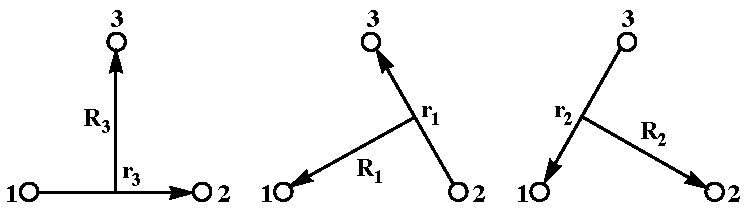
\includegraphics[width=\linewidth]{jacobii.pdf}
	\caption{Three different Jacobi coordinates.}
	\label{fig:2}
\end{figure}

\begin{equation}
\hat{P}_{13} = \left \{ \begin{aligned}
\mathbf{r}' &= \mathbf{x}_2 - \mathbf{x}_3 = \frac{1}{2}\mathbf{r} - \mathbf{R}, \\
\mathbf{R}' &= \mathbf{x}_1 - \frac{1}{2}(\mathbf{x}_3 + \mathbf{x}_2) = -\frac{1}{2}(\frac{3}{2} \mathbf{r} + \mathbf{R}). 
\end{aligned}
\right.
\end{equation}
Similarly, the permutation operator for exchange of particles $(2 \rightarrow 3)$ are defined as

\begin{equation}
\hat{P}_{23} = \left \{ \begin{aligned}
\mathbf{r}'' &= \mathbf{x}_3 - \mathbf{x}_1 = \frac{1}{2}\mathbf{r} + \mathbf{R}, \\
\mathbf{R}'' &= \mathbf{x}_2 - \frac{1}{2}(\mathbf{x}_1 + \mathbf{x}_3) = -\frac{1}{2} (\frac{3}{2} \mathbf{r} - \mathbf{R}).
\end{aligned}
\right.
\end{equation}
For describing permutations in a system with mass-scaled coordinates it is useful to introduce angles defined by the particle masses \cite{Smith1962}\cite{Johnson1980}. If an even permutation $(ijk)$ of the set $(123)$ is considered, then the obtuse angle $\beta_{ij}$ has the properties

\begin{subequations}
	\begin{align}
	&\beta_{ij} = -\beta_{ji}, \quad \beta_{ii} = 0,\\
	&\tan\beta_{ij} = -m_k/\mu,\\
	&d_{i}d_{j} \sin\beta_{ij} = 1,\\
	&d_{i}d_{j} m_{k} \cos\beta_{ij} = -\mu,\\
	&\beta_{12}+\beta_{23}+\beta_{31} = 2\pi
	\end{align}
\end{subequations}
Orthogonal transformations within the coordinate set are then given by 

\begin{equation}
\begin{pmatrix}
\mathbf{r}_j\\
\mathbf{R}_j
\end{pmatrix}
=
\begin{pmatrix}
\cos\beta_{ij} & \sin\beta_{ij}\\
-\sin\beta_{ij} & \cos\beta_{ij}
\end{pmatrix}
\begin{pmatrix}
\mathbf{r}_i\\
\mathbf{R}_i
\end{pmatrix}.
\end{equation}   


\subsection{The Hyperspherical Method}
The next common step in the theoretical framework to describe systems of three particles is to introduce hyperspherical coordinates. The components of the two vectors $\mathbf{r}$ and $\mathbf{R}$ are combined into a single, six-dimensional position vector $\mathbf{q}$. The components of this vector can be regarded as the cartesian components of a point in $\mathbb{R}^{6}$. The motion of the three particle system is thus equivalent to the motion of a single particle, with the reduced mass $\mu$, in six-dimensional Euclidean space. The polar coordinates of this point particle are given by one hyperradial coordinate, $\rho$, and five hyperangular coordinates, collectively labelled $\Omega$. Three of these hyperangles are the Euler angles associated with the orientation of the body fixed frame (i.e., the triangle formed by the three particles) in three-dimensional space, these are called external coordinates. The remaing two hyperangles describe the shape of the triangle, and the hyperradius describes the overall size of the system, these coordinates are the internal coordinates of the system. For the three-body problem, the hyperradius is defined by

\begin{equation}
\rho = \Big(\mathbf{r}^{2} + \mathbf{R}^{2}\Big)^{1/2}, \quad 0\leq \rho < \infty.
\end{equation} 
Hyperspherical coordinates are useful for describing fragmentation problems. Fragmentations processes of the system into any one of the possible channels are described by the hyperradius becoming very large $(\rho \rightarrow \infty)$, while the hyperangles distinguishes between the different fragmentation channels. The hyperradius invariant under both rotations and particle permutation. However, there are various ways to define the hyperangles and they are not in general invariant under particle permutations. The most common choises of parametrizing this hypersphere fall into two distinct categories: Delves coordinates, and (democratic) Smith-Whitten coordinates. 

\subsubsection{Delves Coordinates}
Delves coordinates where originally developed to treat nuclear three-body problems. Numerical difficulties arise with Delves hyper angles when permutation symmetries for three identical particles is considered. Delves coordinates are adapted to collinear atom-diatom collisions and they are regular polar coordinates, where

\begin{subequations}
	\begin{align}
		r_{k} &= \rho \sin{\alpha_{k}}\\
		R_{k} &= \rho \cos{\alpha_{k}}.
	\end{align}
\end{subequations}
The Delves hyperangle $\alpha_{k}$ is then defined by

\begin{equation}
	\alpha_{k} = \arctan\bigg(\frac{r_{k}}{R_{k}}\bigg), \quad 0\leq \alpha_{k} \leq \frac{\pi}{2}.
\end{equation}
This coordinate set corresponds to the reactant arrangement when particle $k$ scatters of the weakly bound particles $i-j$. The other angle in this coordinate set is the angle between the two vectors $\mathbf{r}_{k}$ and $\mathbf{R}_{k}$. It is given by

\begin{equation}
\cos{\theta_{k}} = \frac{\mathbf{r}_{k} \cdot \mathbf{R}_{k}}{r_{k} R_{k}}, \quad  0\leq \theta \leq \pi.
\end{equation}
Now, the massweighted Schr{\"o}dinger equation for the stationary wavefunction $\Psi$ of an n-body system with position vectors $\mathbf{x}_i$ and masses $m_i$, ($i=1,...,N$), interacting pairwise through a potential $V$, is given by

\begin{equation}
-\frac{\hbar^2}{2} \sum_{i=1}^{N} m^{-1}_{i} \nabla^{2}_{\mathbf{x}_{i}} \Psi + V\Psi = E \Psi. 
\end{equation}
Where $\nabla^{2}=\Delta$ is the Laplace operator, which in spherical coordinates reads

\begin{equation}
\Delta = \frac{1}{r^{2}}\frac{\partial}{\partial r} \bigg(r^{2} \frac{\partial}{\partial r}\bigg) - \frac{\hat{L}^{2}}{\hbar^2 r^{2}},
\end{equation}
where $\hat{L}$ is the angular momentum operator associated with the vector $\mathbf{r}$. And

\begin{equation}
\hat{L}^{2} = -\hbar^{2}\Bigg(\frac{1}{\sin{\theta}}\frac{\partial}{\partial \theta} \bigg(\sin{\theta}\frac{\partial}{\partial \theta}\bigg) + \frac{1}{\sin^{2}{\theta}} \frac{\partial^{2}}{\partial \phi^{2}}\Bigg)
\end{equation}
From now on $\hbar = 1$. The kinetic energy for three particles in the mass normalized Jacobi coordinates was given in \eqref{eq:6}. Next follows a derivation the kinetic energy operator in Delves hyperspherical coordinates. The Laplacians for the mass scaled Jacobi vectors are given by

\begin{subequations}
\begin{align}
	\Delta_{r_{k}} &= \frac{1}{r_{k}^2}\frac{\partial}{\partial r_{k}} \bigg( r_{k}^2 \frac{\partial}{\partial r_{k}} \bigg) - \frac{\hat{l}^2_{r_k}}{r_{k}^2} = \frac{2}{r_{k}}\frac{\partial}{\partial r_{k}} + \frac{\partial^2}{\partial r_{k}^{2}} - \frac{\hat{l}^{2}_{r_k}}{r_{k}^2}\\
	\Delta_{R_{k}} &= \frac{1}{R_{k}^2}\frac{\partial}{\partial R_{k}} \bigg( R_{k}^2 \frac{\partial}{\partial R_{k}} \bigg) - \frac{\hat{l}^2_{R_k}}{R_{k}^2} = \frac{2}{R_{k}}\frac{\partial}{\partial R_{k}} + \frac{\partial^2}{\partial R_{k}^{2}} - \frac{\hat{l}^{2}_{R_k}}{R_{k}^2}
\end{align}
\end{subequations}
If spin interactions are excluded the total orbital angular momentum is zero and we have 

\begin{equation}
\hat{l}^{2}_{r_k} = \hat{l}^{2}_{R_k} = -\frac{1}{\sin{\theta}} \frac{\partial}{\partial{\theta}} \bigg( \sin{\theta} \frac{\partial}{\partial{\theta}} \bigg).
\end{equation}
Change of coordinates into Delves polar coordinates results in the following transformations for the partial derivatives of the vector $\mathbf{r}$

\begin{subequations}
\begin{align}
        \frac{\partial}{\partial r}        &= \frac{\partial\alpha}{\partial r} \frac{\partial}{\partial\alpha} +  \frac{\partial\rho}{\partial r} \frac{\partial}{\partial\rho} = \frac{1}{\rho}\cos{\alpha}\frac{\partial}{\partial \alpha} + \sin{\alpha}\frac{\partial}{\partial \rho}, \\
        \frac{\partial^2}{\partial r^2} &= \bigg( \frac{1}{\rho} \cos\alpha \frac{\partial}{\partial\alpha} + \sin\alpha \frac{\partial}{\partial\rho}\bigg) \bigg( \frac{1}{\rho} \cos\alpha \frac{\partial}{\partial\alpha} + \sin\alpha \frac{\partial}{\partial\rho}\bigg) \nonumber \\
                                                     &= \frac{1}{\rho^2} \cos^2\alpha \frac{\partial^2}{\partial\alpha^{2}} - \frac{1}{\rho^2} \sin(2\alpha) \frac{\partial}{\partial\alpha} + \sin^2\alpha \frac{\partial^2}{\partial\rho^{2}} \nonumber \\
                                                     &+ \frac{1}{\rho} \cos^2\alpha \frac{\partial}{\partial\rho} + \frac{1}{\rho} \sin(2\alpha) \frac{\partial^2}{\partial\alpha \partial\rho}.
\end{align}
\end{subequations}
Similarly, the partial derivatives with respect to the vector $\mathbf{R}$ transform as

\begin{subequations}
\begin{align}
        \frac{\partial}{\partial R}        &= \frac{\partial\alpha}{\partial R} \frac{\partial}{\partial\alpha} +  \frac{\partial\rho}{\partial R} \frac{\partial}{\partial\rho} = -\frac{1}{\rho}\sin{\alpha}\frac{\partial}{\partial \alpha} + \cos{\alpha}\frac{\partial}{\partial \rho},  \\
        \frac{\partial^2}{\partial R^2}&= \bigg( -\frac{1}{\rho} \sin\alpha \frac{\partial}{\partial\alpha} + \cos\alpha \frac{\partial}{\partial\rho}\bigg)  \bigg( -  \sin\alpha \frac{\partial}{\partial\alpha} + \cos\alpha \frac{\partial}{\partial\rho}\bigg) \nonumber \\
                                                    &= \frac{1}{\rho^2} \sin^2\alpha\frac{\partial^2}{\partial\alpha^{2}} + \frac{1}{\rho^2} \sin(2\alpha)\frac{\partial}{\partial\alpha} + \cos^2\alpha \frac{\partial^2}{\partial \rho^2} \nonumber \\
                                                    &+\frac{1}{\rho}\sin^2\alpha\frac{\partial}{\partial \rho}- \frac{1}{\rho} \sin(2\alpha) \frac{\partial^2}{\partial\alpha \partial\rho}.
\end{align}
\end{subequations}
Finally, the sum of the two Laplacian operators now reads 

\begin{align}
	\Delta_{r} + \Delta_{R} &= \frac{2}{r}\frac{\partial}{\partial r} +  \frac{2}{R} \frac{\partial}{\partial R}  +\frac{\partial^2}{\partial r^{2}} + \frac{\partial^2}{\partial R^{2}} - \frac{\hat{l}^{2}_{r}}{r^2} - \frac{\hat{l}^{2}_{R}}{R^2} \nonumber \\
									&= \frac{4}{\rho^2} \cot(2\alpha) \frac{\partial}{\partial\alpha} + \frac{5}{\rho} \frac{\partial}{\partial\rho} + \frac{1}{\rho^2} \frac{\partial^2}{\partial\alpha^2} + \frac{\partial^2}{\partial\rho^2} \nonumber \\
									&+ \frac{4}{\rho^2 \sin^2(2\alpha)\sin(\theta)} \frac{\partial}{\partial\theta} \bigg( \sin(\theta) \frac{\partial}{\partial{\theta}} \bigg) \nonumber \\
									&= \frac{1}{\rho^5}\frac{\partial}{\partial\rho} \bigg( \rho^5 \frac{\partial}{\partial\rho} \bigg) + \frac{1}{\rho^2 \sin^2(2\alpha)}  \bigg( \frac{\partial}{\partial\alpha} \sin^2(2\alpha) \frac{\partial}{\partial\alpha} + \frac{4}{\sin\theta} \frac{\partial}{\partial\theta} \bigg).
\end{align}
Thus in Delves hypersherical coordinates the Schr{\"o}dinger equation is given by 

\begin{equation}
\big(\hat{T}_{\rho} + \hat{T}_{\alpha_{k}} + \hat{T}_{\theta} + V(\rho,\Omega)\big) \Psi = E\Psi, 
\end{equation}
where $\hat{T}_{\rho}$ is the hyperradial kinetic energy operator,

\begin{align}
\hat{T}_{\rho} &= -\frac{\hbar^2}{2m} \Big[ \frac{1}{\rho^5}\frac{\partial}{\partial\rho} \Big( \rho^5 \frac{\partial}{\partial\rho} \Big)  \Big] \nonumber\\ 
&= -\frac{\hbar^2}{2m} \Big[ \rho^{-5/2} \Big( \rho^{5/2} \frac{5}{\rho} \frac{\partial}{\partial\rho} + \rho^{5/2} \frac{\partial^2}{\partial\rho^2} \Big) \rho^{-5/2} \rho^{5/2} \Big]\nonumber\\
&= -\frac{\hbar^2}{2m} \rho^{-5/2} \Big[  -\frac{15}{4} \frac{1}{\rho^2} + \frac{\partial^2}{\partial\rho^2} \Big] \rho^{5/2},
\end{align}
$\hat{T}_{\alpha}$ is the kinetic energy operator for the Delves angle $\alpha$,

\begin{align}
\hat{T}_{\alpha} &= -\frac{1}{2\mu}  \frac{1}{\rho^2 \sin^2(2\alpha)}  \bigg[ \frac{\partial}{\partial\alpha} \sin^2(2\alpha) \frac{\partial}{\partial\alpha} \bigg]\nonumber\\ 
&= -\frac{1}{2\mu} \frac{1}{\rho^2} \bigg[ \frac{\partial^2}{\partial\alpha^2} + 4\cot(2\alpha) \frac{\partial}{\partial\alpha} \bigg]\nonumber\\
&= -\frac{1}{2\mu} \frac{1}{\rho^2} \bigg[ \sin^{-1}(2\alpha) \bigg(\sin(2\alpha)\frac{\partial^2}{\partial\alpha^2} + 4\cos(2\alpha) \frac{\partial}{\partial\alpha} \bigg) \sin^{-1}(2\alpha) \sin(2\alpha) \bigg]\nonumber\\
&= -\frac{1}{2\mu} \frac{1}{\rho^2}\sin^{-1}(2\alpha) \bigg[ \frac{\partial^2}{\partial\alpha^2} + 4 \bigg] \sin(2\alpha),
\end{align} 
and $\hat{T}_{\theta}$ is the kinetic energy operator containing the angular momentum operators for the Jacobi vectors,

\begin{align}                  
\hat{T}_{\theta} &= -\frac{1}{2\mu} \bigg[ \frac{4}{\rho^2 \sin^2(2\alpha)\sin(\theta)} \frac{\partial}{\partial\theta} \bigg( \sin(\theta) \frac{\partial}{\partial\theta} \bigg) \bigg]\nonumber\\ 
                      	&= -\frac{1}{2\mu} \bigg[ \frac{1}{\rho^2 \sin^2\alpha\cos^2\alpha\sin\theta} \frac{\partial}{\partial\theta} \bigg( \sin\theta \frac{\partial}{\partial\theta} \bigg) \bigg]
\end{align}
The Hamiltonian operator is given by

\begin{equation}
H_0 = \hat{T}_{\rho} + \hat{T}_{\alpha} + \hat{T}_{\theta} + V(\rho,\Omega).
\end{equation}                      		
Removal of first derivatives with respect to $\rho$ and $\alpha$ is possible by writing the wavefunction as $\Psi = \rho^{-5/2}(\sin(2\alpha))^{-1}\psi$. The coresponding transformation of the Hamiltonian is then


\begin{align}
	H-V &= \rho^{5/2}\sin(2\alpha) (H_0-V) \rho^{-5/2}(\sin(2\alpha))^{-1}\nonumber\\
	    &= -\frac{1}{2\mu} \bigg[ \frac{\partial^2}{\partial\rho^2} - \frac{15}{4\rho^2} + \frac{1}{\rho^2}\bigg( \frac{\partial^2}{\partial\alpha^2} + 4 + \frac{1}{\sin^2\alpha\cos^2\alpha\sin\theta} \frac{\partial}{\partial\theta} \bigg( \sin\theta \frac{\partial}{\partial\theta} \bigg) \bigg) \bigg]\nonumber\\
	    &= -\frac{1}{2\mu} \bigg[ \frac{\partial^2}{\partial\rho^2} + \frac{1}{\rho^2}\bigg( \frac{\partial^2}{\partial\alpha^2} + \frac{1}{\sin^2\alpha\cos^2\alpha\sin\theta} \frac{\partial}{\partial\theta} \bigg( \sin\theta \frac{\partial}{\partial\theta} \bigg) \bigg) + \frac{1}{4\rho^2} \bigg]\nonumber\\
	    &= -\frac{1}{2\mu}\frac{\partial^2}{\partial\rho^2} + \frac{\Lambda^2 - 1/4}{2\mu\rho^2},
\end{align}   
where $\Lambda^2$ is the hyperangular kinetic energy, also called the grand angular momentum operator since it is the angular momentum in this six dimensional space, it is in this case given by 

\begin{equation}
\Lambda^2 = -\frac{\partial^2}{\partial\alpha^2} - \frac{1}{\sin^2\alpha\cos^2\alpha\sin\theta} \frac{\partial}{\partial\theta} \bigg( \sin\theta \frac{\partial}{\partial\theta}\bigg).
\end{equation}
The volume element is proportional to $\rho^5\sin^2\alpha\cos^2\alpha\sin\theta d\rho d\alpha d\theta$. 
%TODO Boundary conditions:
The wavefunction needs to be square-integrable, so $\Psi = 0$ at $\rho=0$ and $\alpha = 0 $ or $\pi$. Further, 

\begin{subequations}
\begin{align*}
	\psi(0,\alpha,\theta) &= 0\\
	\psi(\rho,0,\theta)    &= \psi(\rho,\frac{\pi}{2},\theta) = 0\\
	\frac{\partial\psi}{\partial\theta}\bigg\rvert_{\theta = 0} &= \frac{\partial\psi}{\partial\theta}\bigg\rvert_{\theta = \pi} = 0
\end{align*}   
\end{subequations} 

\subsubsection{Smith-Whitten Coordinates}\label{smith}
%TODO Principel axis methods are characterized by the use of a single hyperspherical coordinate system that treats all three arragements of particles equivalently. 

In this section, we show how the three-body system can be represented in a symmetric way. The derivation of the Hamiltonian for this representation is described using a modified set of Smith-Whitten -- or democratic -- coordinates. 

At any instant, three particles form a plane in $\mathbb{R}^3$. If we consider this plane to be the x-y plane, and define the internal motion of the particles within this plane in terms of  hyperspherical coordinates, our coordinate system must rotate in this plane. That is, we use a body-fixed coordinate system $XYZ$, which rotates with respect to the space fixed axis $X'Y'Z'$. [Details](spatial rotation). The internal coordinates $\rho$, $\Theta$, and $\Phi$ determine the size and shape of the triangle formed by the three particle system. With the $z$-axis perpendicular to the plane, Smith and Whitten [ref] defined these as   

\begin{subequations}
\begin{align*}
	r_x &= \rho \cos(\Theta)\cos(\Phi),\\
	r_y &= -\rho \sin(\Theta)\sin(\Phi),\\
	r_z &= 0\\
	R_x &= \rho \cos(\Theta)\sin(\Phi),\\
	R_y &= \rho \sin(\Theta)\cos(\Phi),\\
	R_z &= 0.
\end{align*}   
\end{subequations}
The distance between the particles are given by

\begin{align}
	x_3 = d_3 \mid\mathbf{r}_{3}\mid &= \frac{\rho d_3}{2^{1/2}}\big[1+\cos(2\Theta)\cos(2\Phi_3)\big]^{1/2}\\
	x_1 = d_1 \mid\mathbf{r}_{1}\mid &= d_1 \big[\cos^2\beta_{31}\mathbf{r}^2_{3} + \sin^2\beta_{31}\mathbf{R}^2_3 + 2\sin\beta_{31}\cos\beta_{31}\mathbf{r}_3\cdot\mathbf{R}_3\big]^{1/2}\\ \notag
	&= \frac{d_1\rho}{2^{1/2}} \big[\cos^2\beta_{31}(1 + \cos(2\Theta)\cos(2\Phi_3))\\ \notag
	&+ \sin^2\beta_{31}(1 - \cos(2\Theta)\cos(2\Phi_3))\\ \notag
	&+ 2\sin\beta_{31}\cos\beta_{31}\cos(2\Theta)\sin(2\Phi_3)\big]^{1/2}\\ \notag
	&= \frac{d_1\rho}{2^{1/2}} \big[1 + \cos(2\Theta)\big(\cos(\Phi_3)\cos(2\beta_{31}) + \sin(2\Phi_3)\sin(2\beta_{31})\big)\big]^{1/2}\\ \notag
	&= \frac{d_1\rho}{2^{1/2}}\big[1 + \cos(2\Theta)\cos(2\Phi_3 - 2\beta_{31})\big]^{1/2}\\ \notag
	&= \frac{d_1\rho}{2^{1/2}}\big[1 + \cos(2\Theta)\cos(2\Phi_1)\big]^{1/2}\\ \notag
	x_2 = d_2 \mid\mathbf{r}_{2}\mid
	&= d_2 \big[\cos^2\beta_{23}\mathbf{r}^2_{3} + \sin^2\beta_{23}\mathbf{R}^2_3 - 2\sin\beta_{23}\cos\beta_{23}\mathbf{r}_3\cdot\mathbf{R}_3\big]^{1/2}\\ \notag
	&= \frac{d_2\rho}{2^{1/2}} \big[1 + \cos(2\Theta)\big(\cos(\Phi_3)\cos(2\beta_{23}) - \sin(2\Phi_3)\sin(2\beta_{23})\big)\big]^{1/2}\\ \notag
	&= \frac{d_1\rho}{2^{1/2}}\big[1 + \cos(2\Theta)\cos(2\Phi_3 + 2\beta_{23})\big]^{1/2}\\ \notag
	&= \frac{d_1\rho}{2^{1/2}}\big[1 + \cos(2\Theta)\cos(2\Phi_2)\big]^{1/2}
\end{align}
Thus, $\Phi_j = \Phi_i-\beta_{ij}$ and

\begin{equation}
	x_k = \frac{d_k\rho}{2^{1/2}}\big[1 + \cos(2\Theta)\cos(2\Phi_k)\big]^{1/2}.
\end{equation}
Now we choose $\Phi_3=\Phi$

\begin{align}
	x_3 &= \frac{\rho d_3}{2^{1/2}}\big[1+\cos(2\Theta)\cos(2\Phi)\big]^{1/2}\\
	x_1 &= \frac{d_1\rho}{2^{1/2}}\big[1 + \cos(2\Theta)\cos(2\Phi + \epsilon_1)\big]^{1/2}\\
	x_2 &= \frac{d_1\rho}{2^{1/2}}\big[1 + \cos(2\Theta)\cos(2\Phi + \epsilon_2)\big]^{1/2}
\end{align}
where

\begin{align}
	\epsilon_1 &= -2\tan^{-1}(-m_2/\mu)\\
	\epsilon_2 &= 2\tan^{-1}(-m_1/\mu)
\end{align}
Now for three identical particles we get

\begin{align}
x_3 &= \frac{\rho}{3^{1/4}}\big[1+\cos(2\Theta)\cos(2\Phi)\big]^{1/2}\\
x_1 &= \frac{\rho}{3^{1/4}}\big[1 + \cos(2\Theta)\cos(2\Phi - 4\pi/3)\big]^{1/2}\\
x_2 &= \frac{\rho}{3^{1/4}}\big[1 + \cos(2\Theta)\cos(2\Phi + 4\pi/3)\big]^{1/2}
\end{align}

Now, with $\phi_k = \pi/2-2\Phi_k$, we get $\phi_j=\phi_i+2\beta_{ij}$, where ($-7\pi/2 \leq \phi_k < \pi/2$). Now with $2\beta_{ij} = -2\eta_{ij}$ and

\begin{align}
	&\eta_{ij} = -\eta_{ji}, \quad \eta_{ii} = 0,\\
	&\tan\eta_{ij} = m_k/\mu,\\
	&\eta_{12}+\eta_{23}+\eta_{31} = \pi
\end{align} 
We get

\begin{equation}
x_k = \frac{d_k\rho}{2^{1/2}}\big[1 + \sin\theta\sin\phi_k\big]^{1/2}.
\end{equation}

\begin{align}
x_3 &= \frac{d_3\rho}{2^{1/2}}\big[1+\sin\theta\sin\phi\big]^{1/2}\\
x_1 &= \frac{d_1\rho}{2^{1/2}}\big[1 + \sin\theta\sin(\phi-\varphi_1)\big]^{1/2}\\
x_2 &= \frac{d_1\rho}{2^{1/2}}\big[1 + \sin\theta\sin(\phi + \varphi_2)\big]^{1/2}
\end{align}

\begin{align}
\varphi_1 &= 2\tan^{-1}(m_2/\mu)\\
\varphi_2 &= 2\tan^{-1}(m_1/\mu)
\end{align}
Now we redefine $\phi'_k = \phi_k+7\pi/2$, so that the range is $0 \leq \phi'_k < 4\pi$. Then $\sin\phi_k = \cos\phi'_k$. We finally get ($2\Phi = 4\pi - \phi'$)

\begin{align}
x_3 &= \frac{d_3\rho}{2^{1/2}}\big[1+\sin\theta\cos\phi'\big]^{1/2}\\
x_1 &= \frac{d_1\rho}{2^{1/2}}\big[1 + \sin\theta\cos(\phi'-\varphi_1)\big]^{1/2}\\
x_2 &= \frac{d_1\rho}{2^{1/2}}\big[1 + \sin\theta\cos(\phi' + \varphi_2)\big]^{1/2}.
\end{align}
This is the same expression as Blume and Wang get, however the define there angles slightly different. Our interval is two times Blumes interval 

The area of the triangle formed by the three particles is the length of the vector given by

\begin{equation}
	\mathbf{A}=\frac{1}{2} (\mathbf{r}\times \mathbf{R})
\end{equation}

\begin{align}
&A =\frac{1}{2} (r_x R_y - r_y R_x) = \frac{1}{4}\rho^2\sin(2\Theta)\\
&\sin2\Theta = 4A/\rho^2
\end{align}
Since both the area and the hyperradius are positive quantities the angle must be in the range, $0\leq \Theta \leq \pi/4$. For some reason $0\leq \Phi < 2\pi$. The transformed coordinates then have the range $0\leq \theta \leq \pi/2$ and 

To describe how rotations of the BF system affects the derivatives in the SF system, introduce the infinitesimal rotations $\mathbf{\omega}$. The velocities of the SF system vectors are given by    

\begin{subequations}
	\begin{align*}
	 \dot{\mathbf{r}}' = \dot{\mathbf{r}} + \mathbf{\omega} \times \mathbf{r}\\
	 \dot{\mathbf{R}}' = \dot{\mathbf{R}} + \mathbf{\omega} \times \mathbf{R}\\
	\end{align*}   
\end{subequations} 

which is given explicitly by

\begin{align}
\begin{pmatrix}
       \dot{r}'_x \\
       \dot{r}'_y \\
       \dot{r}'_z \\
       \dot{R}'_x \\
       \dot{R}'_y \\
       \dot{R}'_z\\
 \end{pmatrix} 
 &= 
 \begin{pmatrix*}[c]
       \partial_{\rho} r_x & \partial_{\Theta} r_x & \partial_{\Theta} r_x & 0 & r_z & -r_y\\
       \partial_{\rho} r_y & \partial_{\Theta} r_y & \partial_{\Theta} r_y & -r_z & 0 & r_x\\
       \partial_{\rho} r_z & \partial_{\Theta} r_z & \partial_{\Theta} r_z & r_y & -r_x & 0\\
       \partial_{\rho} R_x & \partial_{\Theta} R_x & \partial_{\Theta} R_x & 0 & R_z & -R_y\\
       \partial_{\rho} R_y & \partial_{\Theta} R_y & \partial_{\Theta} R_y & -R_z & 0 & R_x\\
       \partial_{\rho} R_z & \partial_{\Theta} R_z & \partial_{\Theta} R_z & R_y & -R_x & 0\\
     \end{pmatrix*}
     \begin{pmatrix}
     \dot{\rho}\\
     \dot{\Theta}\\
     \dot{\Phi}\\
     \omega_x\\
     \omega_y\\
     \omega_z\\
     \end{pmatrix} \notag \\
     &=
     \begin{pmatrix*}[c]
       cc & -sc & -cs & 0 & 0 & ss\\
       -ss & -cs & -sc & 0 & 0 & cc\\
       0 & 0 & 0 & -ss & -cc & 0\\
       cs & -ss & cc & 0 & 0 & -sc\\
       sc & cc & -ss & 0 & 0 & cs\\
       0 & 0 & 0 & sc & -cs & 0\\
     \end{pmatrix*}
     \begin{pmatrix}
     \dot{\rho}\\
     \rho \dot{\Theta}\\
     \rho \dot{\Phi}\\
     \rho \omega_x\\
     \rho \omega_y\\
     \rho \omega_z\\
     \end{pmatrix}\\
\end{align}
In matrix notation:

\begin{equation}
	\dot{\mathbf{q}}' = \hat{A}\dot{\mathbf{q}},
\end{equation} 
where     
     
\begin{equation}
\dot{\mathbf{q}}' =
\begin{pmatrix}
\dot{r}'_x \\
\dot{r}'_y \\
\dot{r}'_z \\
\dot{R}'_x \\
\dot{R}'_y \\
\dot{R}'_z\\
\end{pmatrix},
\dot{\mathbf{q}} =
\begin{pmatrix}
\dot{\rho}\\
\dot{\Theta}\\
\dot{\Phi}\\
\omega_x\\
\omega_y\\
\omega_z\\
\end{pmatrix} \notag \\
\end{equation}

     
The arclength is given by

\begin{equation}
s = \int_{a}^{b} \| \dot{\mathbf{q}}' \| dt = \int_{a}^{b} \sqrt{ \dot{\mathbf{q}}'^{T} \dot{\mathbf{q}}'}\\ dt
\end{equation}

and

\begin{equation}
(ds)^2 = (d\mathbf{q}')^{T}(d\mathbf{q}') = d\mathbf{q}^{T} \hat{A}^{T} \hat{A}d\mathbf{q} = d\mathbf{q}^{T} \mathbf{g} d\mathbf{q},
\end{equation}
where $\mathbf{g}$ is the metric tensor

\begin{equation}
\mathbf{g}=
\begin{pmatrix}
\mathbf{G} & \mathbf{C}\\
\mathbf{C}^T & \mathbf{K}
\end{pmatrix}
\end{equation}
where the submatrices $\mathbf{G}$, $\mathbf{K}$ and $\mathbf{C}$ are 

\begin{align}
\mathbf{G} &=
\begin{pmatrix}
1 & 0      & 0\\
0 & \rho^2 & 0\\
0 & 0      & \rho^2
\end{pmatrix}\\
\mathbf{K} &=
\rho^2
\begin{pmatrix}
\sin^2\Theta & 0            & 0\\
0            & \cos^2\Theta & 0\\
0            & 0            & 1
\end{pmatrix}\\
\mathbf{C} &=
-\rho^2\sin^2(2\Theta)
\begin{pmatrix}
0 & 0 & 0\\
0 & 0 & 0\\
0 & 0 & 1
\end{pmatrix}
\end{align}
the inverse of the metric tensor $\mathbf{g}^{-1}$
\begin{equation}
\mathbf{g}^{-1}=
\begin{pmatrix}
\mathbf{V} & \mathbf{W}\\
\mathbf{W}^T & \mathbf{U}
\end{pmatrix}
\end{equation}
where the submatrices $\mathbf{V}$, $\mathbf{W}$ and $\mathbf{U}$ are 

\begin{align}
\mathbf{V} &=
\begin{pmatrix}
1 & 0      & 0\\
0 & 1/\rho^2 & 0\\
0 & 0      & 1/\rho^2\cos^2(2\Theta)
\end{pmatrix}\\
\mathbf{U} &=
\frac{1}{\rho^2}
\begin{pmatrix}
1/\sin^2\Theta & 0            & 0\\
0            & 1/\cos^2\Theta & 0\\
0            & 0            & 1/\cos^2(2\Theta)
\end{pmatrix}\\
\mathbf{W} &=
\frac{\sin(2\Theta)}{\rho^2\cos^2(2\Theta)}
\begin{pmatrix}
0 & 0 & 0\\
0 & 0 & 0\\
0 & 0 & 1
\end{pmatrix}
\end{align}

The determinant of the metric tensor is given by

\begin{align}
g &=
\mid\mathbf{g}\mid=
\begin{vmatrix}
\mathbf{G} & \mathbf{C}\\
\mathbf{C}^T & \mathbf{K}
\end{vmatrix}
=
\begin{vmatrix}
\mathbf{G} & \mathbf{C}\\
0 & \mathbf{K} - \mathbf{C}^T \mathbf{G}^{-1} \mathbf{C}
\end{vmatrix}\\
  &=
\mid \mathbf{G} \mid \cdot \mid\mathbf{K} - \mathbf{C}^T \mathbf{G}^{-1} \mathbf{C} \mid
=
\frac{\rho^{10}}{16}\sin^2(4\Theta)
\end{align}

\begin{equation}
	\sqrt{g}=\frac{\rho^5}{4}\sin(4\Theta)
\end{equation}

The kinetic energy operator of a particle with mass $\mu$ in a curvilinear coordinate system of $N$ dimensions is given by

\begin{equation}
	T = -\frac{\hbar^2}{2\mu} \sum_{i=1}^{N} \sum_{j=1}^{N} \frac{1}{\sqrt{g}} \frac{\partial}{\partial q_i} \Big(\sqrt{g} g^{ij} \frac{\partial}{\partial q_j}\Big)
\end{equation}
where $g^{ij}$ is the inverse metric tensor. The momentum vector is given by

\begin{equation}
	\mathbf{p} = i\hbar 
	\begin{pmatrix}
		\partial/\partial q_1\\
		\vdots\\
		\partial/\partial q_N\\
	\end{pmatrix}
\end{equation}

With $\mathbf{\omega}$ expressed in Euler angles 

\begin{equation}
\mathbf{\omega} = 
\begin{pmatrix}
	d\Omega_x\\
	d\Omega_y\\
	d\Omega_z
\end{pmatrix}
\end{equation}

we get the kinetic energy

\begin{align*}
	-\frac{1}{\hbar^2}\hat{T} &= -\frac{1}{2\mu \rho^5 \sin(4\Theta)} \mathbf{p}^T \Big(\rho^5 \sin(4\Theta) \mathbf{g}^{-1}\Big) \mathbf{p}\\
	  &= \frac{1}{2\mu \rho^5 \sin(4\Theta)}\Bigg[ \frac{\partial}{\partial \rho} \Bigg(\rho^5 \sin(4 \Theta) \frac{\partial}{\partial \rho}\Bigg) + \frac{\partial}{\partial \Theta}\Bigg(\rho^3\sin(4\Theta)\frac{\partial}{\partial\Theta}\Bigg)\\ &+\frac{\partial}{\partial\Phi}\Bigg(2\rho^3\tan(2\Theta)\frac{\partial}{\partial\Phi} + 2\tan^2(2\Theta)\cos(2\Theta)\frac{\partial}{\partial\Omega_z}\Bigg)\\
	  &+\frac{\partial}{\partial\Omega_x}\Bigg(4\rho^3\cot(\Theta)\cos(2\Theta)\frac{\partial}{\partial\Omega_x}\Bigg)\\
	  &+\frac{\partial}{\partial\Omega_y}\Bigg(4\rho^3\tan(2\Theta)\cos(2\Theta)\frac{\partial}{\partial\Omega_y}\Bigg)\\
	  &+\frac{\partial}{\partial\Omega_z}\Bigg(2\rho^3\tan^2(2\Theta)\frac{\partial}{\partial\Phi}+2\rho^3\tan(2\Theta)\frac{\partial}{\partial\Omega_z}\Bigg)\Bigg]\\
	  &=\frac{1}{2\mu}\Bigg[\frac{1}{\rho^5}\frac{\partial}{\partial\rho}\Bigg(\rho^5\frac{\partial}{\partial\rho}\Bigg) + \frac{1}{\rho^2\sin(4\Theta)}\frac{\partial}{\partial\Theta}\Bigg(\sin(4\Theta)\frac{\partial}{\partial\Theta}\Bigg)\\
	  &+\frac{1}{\rho^2\cos^2(2\Theta)}\frac{\partial^2}{\partial\Phi^2} + \frac{\sin(2\Theta)}{\rho^2\cos^2(2\Theta)}\frac{\partial}{\partial\Phi}\frac{\partial}{\partial\Omega_z}\\
	  &+\frac{1}{\rho^2\sin^2(\Theta)}\frac{\partial^2}{\partial\Omega^2_x} + \frac{1}{\rho^2\cos^2(\Theta)}\frac{\partial^2}{\partial\Omega^2_y} + \frac{\sin(2\Theta)}{\rho^2\cos^2(2\Theta)}\frac{\partial}{\partial\Omega_z}\frac{\partial}{\partial\Phi}\\
	  &+ \frac{1}{\rho^2\cos^2(2\Theta)}\frac{\partial^2}{\partial\Omega^2_z}\Bigg]\\
	  &=\frac{1}{2\mu\rho^5}\frac{\partial}{\partial\rho}\Bigg(\rho^5\frac{\partial}{\partial\rho}\Bigg) + \frac{1}{2\mu\rho^2}\Bigg[\frac{1}{\sin(4\Theta)}\frac{\partial}{\partial\Theta}\Bigg(\sin(4\Theta)\frac{\partial}{\partial\Theta}\Bigg)\\
	  &+\frac{1}{\cos^2(2\Theta)}\frac{\partial^2}{\partial\Phi^2} \Bigg]+\frac{1}{2\mu\rho^2}\Bigg[\frac{1}{\sin^2(\Theta)}\frac{\partial^2}{\partial\Omega^2_x} + \frac{1}{\cos^2(\Theta)}\frac{\partial^2}{\partial\Omega^2_y} + \frac{1}{\cos^2(2\Theta)}\frac{\partial^2}{\partial\Omega^2_z}\\
	  &+ \frac{2\sin(2\Theta)}{\cos^2(2\Theta)}\frac{\partial}{\partial\Phi}\frac{\partial}{\partial\Omega_z}\Bigg].
\end{align*}

The volume element in a general coordinate system of  N dimensions is given by

\begin{equation}
d^Nv = g^{1/2}\prod_{i=1}^{N} dq_i
\end{equation}
The Euler angles are given by

\begin{equation}
\begin{pmatrix}
d\Omega_x\\
d\Omega_y\\
d\Omega_z
\end{pmatrix}
=
\mathbf{A}\begin{pmatrix}
d\alpha\\
d\beta\\
d\gamma
\end{pmatrix}
\end{equation}
where

\begin{equation}
\mathbf{A}=
	\begin{pmatrix}
		-\sin\beta\cos\gamma & \sin\gamma & 0\\
		\sin\beta\sin\gamma  & \cos\gamma & 0\\
		\cos\beta 			 & 0          & 1
	\end{pmatrix}
\end{equation}

\begin{equation}
d\mathbf{q} =
\begin{pmatrix}
d\rho\\
d\Theta\\
d\Phi\\
d\Omega_x\\
d\Omega_y\\
d\Omega_z\\
\end{pmatrix},
d\mathbf{q}' =
\begin{pmatrix}
d\rho\\
d\Theta\\
d\Phi\\
d\alpha\\
d\beta\\
d\gamma\\
\end{pmatrix} \notag \\
\end{equation}

\begin{equation}
	ds^2 = (d\mathbf{q})^T\mathbf{g}d\mathbf{q} = (d\mathbf{q}')^T\mathbf{g}'d\mathbf{q}'
\end{equation}
with

\begin{equation}
	\mathbf{B} = 
	\begin{pmatrix}
		\mathbf{I} & 0\\
		0      & \mathbf{A}
	\end{pmatrix}
\end{equation}

\begin{equation}
	\mathbf{g}'=\mathbf{B}^T\mathbf{g}\mathbf{B}
\end{equation}
and the determinant is then

\begin{equation}
g'^{1/2}=(\mid\mathbf{B}\mid^2 \mid\mathbf{g}\mid)^{1/2} = (\mid\mathbf{A}\mid^2 \mid\mathbf{g}\mid)^{1/2}
  = \frac{\rho^5}{4}\sin(4\Theta)\sin\beta
\end{equation}

In our set up we thus get 

\begin{equation}
d^6v = g^{1/2}\prod_{i=1}^{6} dq_i = \frac{\rho^5}{4}\sin(4\Theta)\sin\beta d\rho d\Theta d\Phi d\alpha d\beta d\gamma
\end{equation}

Now, we make a transformation of the angles (Kuppermann)

\begin{align*}
	\Theta &= \pi/4-\theta/2\\
	\Phi &= \pi/4-\phi/2
\end{align*}

and

\begin{align*}
	\frac{\partial}{\partial\Theta} &= -2\frac{\partial}{\partial\theta}\\ 						\frac{\partial}{\partial\Phi} &= -2\frac{\partial}{\partial\phi}\\ 		
\end{align*}

\begin{align*}
	&\sin(4\Theta)   =\sin(2\theta)\\
	&\cos^2(2\Theta) =\sin^2(\theta)\\
	&\sin^2(2\Theta) =\cos^2(\theta)\\
	&\cos^2\Theta    =\frac{1}{2}(1+\sin\theta)\\
	&\sin^2\Theta    =\frac{1}{2}(1-\sin\theta)\\
\end{align*}
The corresponding volume element is then

\begin{equation}
	d^6 v = \frac{1}{8}\rho^5 \sin\theta\cos\theta\sin\beta d\rho d\theta d\phi d\alpha d\beta d\gamma
\end{equation}

Now with

\begin{equation}
	\mathbf{P} = 
	-i\hbar
	\begin{pmatrix}
	\partial/\partial\rho\\
	\partial/\partial\theta\\
	\partial/\partial\phi
	\end{pmatrix}
	=
	\begin{pmatrix}
	P_{\rho}\\
	P_{\theta}\\
	P_{\phi}
	\end{pmatrix}
\end{equation}
and

\begin{equation}
	\mathbf{J} = 
	-i\hbar
	\begin{pmatrix}
	\partial/\partial\Omega_x\\
	\partial/\partial\Omega_y\\
	\partial/\partial\Omega_z
	\end{pmatrix}
	=
	\begin{pmatrix}
	J_x\\
	J_y\\
	J_z
	\end{pmatrix}
\end{equation}

The kinetic energy operator then becomes

\begin{align*}
	\hat{T} &=-\frac{\hbar^2}{2\mu}\Bigg[\frac{1}{\rho^5}\frac{\partial}{\partial\rho}\rho^5\frac{\partial}{\partial\rho} + \frac{4}{\rho^2}\Bigg(\frac{1}{\sin(2\theta)}\frac{\partial}{\partial\theta}\sin(2\theta)\frac{\partial}{\partial\theta}\\
	&+\frac{1}{\sin^2(\theta)}\frac{\partial^2}{\partial\phi^2} \Bigg)\Bigg]-\frac{1}{\mu\rho^2}\Bigg[\frac{J^2_x}{(1-\sin\theta)} + \frac{J^2_y}{(1+\sin\theta)} +\frac{J^2_z}{2\sin^2\theta}\Bigg]\\
	&+ \frac{4i\hbar\cos\theta J_z}{2\mu\rho^2\sin^2\theta}\frac{\partial}{\partial\phi}
\end{align*}

If we only consider $J=0$ states, the Hamiltonian reduces to 

\begin{equation}
H_{0} = -\frac{\hbar^{2}}{2 \mu} \Bigg[ \frac{1}{\rho^{5}} \frac{\partial}{\partial \rho} \rho^{5} \frac{\partial}{\partial \rho} + \frac{4}{\rho^{2}}\Big( \frac{1}{\sin(2\theta)} \frac{\partial}{\partial \theta} \sin(2\theta) \frac{\partial}{\partial \theta} + \frac{1}{\sin^{2}(\theta)} \frac{\partial^{2}}{\partial \phi^{2}} \Big) \Bigg] + V(\rho, \theta, \phi)
\end{equation}

By making the following transformation of the wave function 
\begin{equation}
\psi = \rho^{5/2} \Psi,
\end{equation}
the Schr{\"o}dinger equation becomes

\begin{equation}
H \psi = E \psi. 
\end{equation}
Where the transformed Hamiltonian operator is given by

\begin{equation}
H = \rho^{5/2}H_{0} \rho^{-5/2}. 
\end{equation}
This transformation removes the first derivative in the hyper radial kinetic-energy operator since

\begin{equation}
T_{\rho} = \rho^{5/2}T_{\rho_{0}}\rho^{-5/2} = \rho^{5/2} \frac{1}{\rho^{5}} \frac{\partial}{\partial \rho} \rho^{5} \frac{\partial}{\partial \rho} \Big( \rho^{-5/2} \Big) = -\frac{15}{4} \frac{1}{\rho^{2}} + \frac{\partial^{2}}{\partial \rho^{2}}
\end{equation}
and we get the final expression for the Hamiltonian

\begin{align}
H &= -\frac{\hbar^{2}}{2 \mu} \Bigg[ -\frac{15}{4} \frac{1}{\rho^{2}} + \frac{\partial^{2}}{\partial \rho^{2}}+ \frac{4}{\rho^{2}}\Big( \frac{1}{\sin(2\theta)} \frac{\partial}{\partial \theta} \sin(2\theta) \frac{\partial}{\partial \theta} + \frac{1}{\sin^{2}(\theta)} \frac{\partial^{2}}{\partial \phi^{2}} \Big) \Bigg] + V(\rho, \theta, \phi)\\
    &= -\frac{\hbar^{2}}{2 \mu \rho^{2} }\frac{\partial^2}{\partial \rho^2} + \frac{\hbar^{2}}{2 \mu \rho^{2} } \Bigg(\Lambda^2 + \frac{15}{4}\Bigg)+ V(\rho, \theta, \phi),
\end{align}
where $\Lambda^2$ is the grand angular momentum operator. 

\subsubsection{Symmetries}
The Smith-Whitten coordinates $\theta$ and $\phi$ are connected to the geometry of the triangle formed by the three particles. If the three particles represent the vertecis of a triangle, $\theta$ will determine its shape, while $\phi$ determines the arrangement of the particles at its vertecis. Now lets determine the eigenvalues and eigenfunctions of the grand angular momentum operator. For the $\phi$ equation we have

\begin{equation}
\frac{\partial^{2}}{\partial \phi^{2}} \me^{ i \nu \phi} = -\nu^{2} \me^{ i \nu \phi}\\,
\end{equation}
so the total eigenfunction can be written

\begin{equation}
f_{\nu n}(\theta,\phi) = g_{n \nu}(\theta) \me^{ i \nu \phi}\\. 
\end{equation}
For a general system we have the symmetry 

\begin{equation}
f_{\nu n}(\theta,\phi = 0) = \Pi f_{\nu n}(\theta,\phi = 2\pi), \qquad \text{for} \qquad \Pi = \pm 1,\\
\end{equation}
the symmetry of a three identical particle system will reduce the interval of $\phi$ to $[0,2\pi/3]$. (symmetry group $C_{3v}$ with irreducible representations $A_{1}$, $A_{2}$, and $E$), we will consider bosons and states with $J=0$ so this leads to vibrational wave functions of $A_{1}$ symmetry and this will reduce the interval of $\phi$ further to $[0,\pi/3]$, so

\begin{equation}
f_{\nu n}(\theta,\phi = 0) = \Pi f_{\nu n}(\theta,\phi =2 \pi/3),  \qquad \text{for} \qquad  \Pi = \pm 1,\\
\end{equation}
where the parity $\Pi = 1$ for bosons. Thus

\begin{equation}
 \me^{ i \nu 2\pi/3} = 1 \quad \Leftrightarrow  \quad \nu = 3n \quad \text{for} \quad n=0,1,2,...\\
\end{equation}
so we get

\begin{equation}
\Lambda^{2} g_{n \nu}(\theta) = -4\Bigg(\frac{1}{\sin(2\theta)} \frac{\partial}{\partial \theta} \sin(2\theta) \frac{\partial}{\partial \theta} - \frac{\nu^{2}}{\sin^{2}(\theta)}\Bigg) g_{n \nu}(\theta) = \lambda_{n \nu} g_{n \nu}(\theta).\\
\end{equation}
The interval for $\theta$ is $[0,\pi/2]$. Lets look at the boundary as $\theta \rightarrow 0$. The small angle approximation leads to

\begin{equation}
\Lambda^{2} \rightarrow -4\Bigg(\frac{1}{\theta} \frac{\partial}{\partial \theta} + \frac{\partial^{2}}{\partial \theta^{2}} - \frac{\nu^{2}}{\theta^{2}}\Bigg) g_{n \nu}(\theta) = \lambda_{n \nu} g_{n \nu}(\theta).\\
\end{equation}
we thus need to solve a differential equation of the form

\begin{equation}
g_{n\nu}''(\theta) + \frac{P(\theta)}{\theta}g_{n\nu}'(\theta) + \frac{Q(\theta)}{\theta^{2}}g_{n\nu}(\theta) = 0,\\
\end{equation}
with

\begin{equation}
P(\theta)=1 \quad \text{and} \quad Q(\theta)= \frac{\lambda_{n \nu}\theta^{2} - 4\nu^{2}}{4}.\\
\end{equation}
Since ref[the differential equation] has a regular singular point at $\theta = 0$ and both $P(\theta)$ and $Q(\theta)$ are analytic functions, we seek a power series solution of the form

\begin{equation}
g_{n\nu}(\theta) = \sum_{k=0}^{\infty} A_{k} \theta^{k+s}, \quad (A_{0} \neq 0).\\
\end{equation}
differentiating

\begin{equation}
g'_{n\nu}(\theta) = \sum_{k=0}^{\infty} (k+s) A_{k} \theta^{k+s-1},\\
\end{equation}


\begin{equation}
g''_{n\nu}(\theta) = \sum_{k=0}^{\infty} (k+s)(k+s-1) A_{k} \theta^{k+s-2},\\
\end{equation}
and substituting into [ref] we get

\begin{align*}
&\sum_{k=0}^{\infty} \Bigg( (k+s)(k+s-1) + (k+s) - \nu^{2}\Bigg) A_{k} \theta^{k+s-2} + \Bigg(\frac{\lambda_{n\nu}}{4}  \Bigg) A_{k} \theta^{k+s} = \\
&\big[ s(s-1) + s -\nu^{2} \big] A_{0} \theta^{s-2} + \sum_{k=1}^{\infty} \Bigg( \big[ (k+s)(k+s-1) + (k+s) - \nu^{2}  \big] A_{k} + \frac{\lambda_{n\nu}}{4} A_{k-2}\Bigg) \theta^{k+s-2}\\
\end{align*}
From $s^{2} - \nu^{2} = 0$ we get the two roots $s = \pm \nu$. Using these roots, we set the coefficients of $\theta^{k+s-2}$ to be zero, and we get the equations

\begin{equation}
\big(k^{2} \pm 2k\nu\big)A_{k} = \frac{\lambda_{n\nu}}{4} A_{k-2}\\
\end{equation} 

The table \ref{table:1} shows the analytically derived eigenvalues in SW-coordinates.

\begin{table}[h!]
	\centering
	\begin{tabular}{||c c c c c c||} 
		\hline
		$\nu=0$ & $\nu=3$ & $\nu=6$ & Total & $\lambda(\lambda+4)$& multiplicity \\ [0.5ex] 
		\hline\hline
		0		& 60     & 192 & 0 & 0 & 1  \\ 
		32	   & 140   & 320 & 32 & 4 & 1  \\
		96     & 252  & 480 & 60 & 6 & 1  \\
		192   & 396  & 672  & 96 & 8 & 1  \\
		320   & 572  & 896  & 140 & 10 & 1  \\
		480   & 780  & 1152 & 192 & 12 & 2  \\  
		672   & 1020 & 1440 & 252 & 14 & 1  \\ [1ex] 
		\hline
	\end{tabular}
	\caption{Analytically derived eigenvalues}
	\label{table:1}
\end{table}

\subsection{Adiabatic hyperspherical method}\label{sec:AHM}
In the following sections we have chosen to work in the set of democratic hyperangles described in \ref{smith}. With these coordinates, the Schr{\"o}dinger equation for the internal coordinates was derived as  

\begin{equation}\label{schrodinger}
\Bigg(-\frac{1}{2 \mu}\frac{\partial^2}{ \partial \rho^2} + \frac{\Lambda^2 + 15/4}{2 \mu \rho^2} + V(\rho,\theta,\phi) \Bigg)\psi(\rho,\theta,\phi) = E\psi(\rho,\theta,\phi),
\end{equation}
with boundary conditions

\begin{align}
\frac{\partial\Phi_{\nu}(\rho;0,\phi)}{\partial \theta} = \frac{\partial\Phi_{\nu}(\rho;\frac{\pi}{2},\phi)}{\partial \theta},\\
\frac{\partial\Phi_{\nu}(\rho;\theta,0)}{\partial \phi} = \frac{\partial\Phi_{\nu}(\rho;\theta,\frac{2\pi}{3})}{\partial \phi},
\end{align}
reflecting three identical particle symmetry. We assume that the interactions $V$ can be written as a sum of pairwise two-body potentials   

\begin{equation}
V(\rho,\theta,\psi) = v(r_{k}) + v(r_{i}) + v(r_{j}).
\end{equation}
The two-body interaction 

\begin{equation}
v(r) = d\cosh^{-2}{(r/r_0)}.
\end{equation}

\begin{align}
r_3 &= 3^{-1/4}\rho [1+\sin \theta \cos \phi]^{1/2} \\
r_1 &= 3^{-1/4}\rho [1+\sin \theta \cos (\phi - 2\pi/3)]^{1/2} \\
r_2 &= 3^{-1/4}\rho [1+\sin \theta \cos (\phi + 2\pi/3)]^{1/2} 
\end{align}
The exact solution to \eqref{schrodinger} can be found by first writing $\psi_{n}(\rho,\theta,\phi)$ as an expansion of radial wavefunctions $F_{\nu n}(\rho)$ and a set of complete, orthonormal channel functions $\Phi_{\nu}(\rho;\theta,\phi)$ that depend parametrically on $\rho$,

\begin{equation}\label{wave}
\psi_{n}(\rho,\theta,\phi) = \sum_{\nu=0}^{\infty} F_{n\nu}(\rho)\Phi_{\nu}(\rho;\theta,\phi).
\end{equation}
The channel functions $\Phi_{\nu}$ are solutions to the hyperangular part of \eqref{schrodinger}

\begin{equation}\label{adiabatic}
 \bigg(\frac{\Lambda^2+15/4}{2 \mu_{3} \rho^2} + V(\rho,\theta,\phi)\bigg) \Phi_{\nu}{(\rho;\theta,\phi)}= U_{\nu}{(\rho)} \Phi_{\nu}(\rho;\theta,\phi),
\end{equation}
and $U_{\nu}(\rho)$ are the resulting effective potental curves obtained by solving this eigenvalue equation at a number of different hyperradii. Substituting \eqref{wave} into \eqref{schrodinger} and projecting out $\Phi_{\nu'}$ by multiplying the conjugate transpose $\Phi_{\nu}^{\dagger}$ to the left and integrating over the hyperanglular coordinates results in an infinite set of coupled differential equation in $\rho$, which reads

\begin{align}\label{fullhamiltonian}
\bigg(-\frac{1}{2 \mu}\frac{\partial^2}{ \partial \rho^2} + U_{\mu}(\rho) - \frac{1}{2\mu}Q_{\mu\mu}(\rho) \bigg)F_{n\mu}(\rho)&\nonumber\\ -\frac{1}{2\mu}\bigg(\sum_{\nu\neq\mu}2P_{\mu\nu}(\rho)\frac{\partial}{\partial\rho} + Q_{\mu\nu}(\rho) \bigg)F_{n\nu}(\rho)& = E_nF_{n\mu}(\rho),
\end{align}
where the nonadiabatic coupling terms $P_{\mu\nu}$ and $Q_{\mu\nu}$ involve partial first and second derivative of the channel functions with respect to $\rho$. They are generated by the $\rho$ dependence of the channel functions and are defined as 

\begin{equation}\label{couplingP}
P_{\mu\nu}(\rho) = \llangle[\Big]  \Phi_{\mu} \Big\lvert \frac{\partial}{\partial\rho} \Big\rvert  \Phi_{\nu} \rrangle[\Big],
\end{equation}
and

\begin{equation}\label{couplingQ}
Q_{\mu\nu}(\rho) = \llangle[\Big]  \Phi_{\mu} \Big\lvert \frac{\partial^2}{\partial\rho^2} \Big\rvert  \Phi_{\nu} \rrangle[\Big],
\end{equation}
where the double brackets denote integration over the two angular coordinates. Integration by parts, the completeness requirement of the channelfunctions together with the antisymmetric properties of the coupling matrix $P_{\mu \nu}$,  i.e. $P_{\mu \nu}= - P_{\nu \mu}$, are used to derive the following relation 

\begin{equation}
Q_{\mu \nu} = \frac{dP_{\mu \nu}}{d\rho} + P^2_{\mu \nu},
\end{equation}
where the square of the coupling matrix $P_{\mu \nu}$ relates to $Q_{\mu \nu}$ through 

\begin{align}
P^2_{\mu \nu} &= \sum_{\sigma}P_{\mu \sigma}P_{\sigma \nu} = \sum_{\sigma}\llangle[\Big] \Phi_{\mu} \Big\lvert \frac{\partial \Phi_{\sigma}}{\partial\rho}  \rrangle[\Big]\llangle[\Big] \Phi_{\sigma} \Big\lvert \frac{\partial \Phi_{\nu}}{\partial\rho}  \rrangle[\Big]\nonumber\\
&=\sum_{\sigma}-\llangle[\Big]\frac{\partial \Phi_{\mu}}{\partial\rho} \Big\lvert  \Phi_{\sigma} \rrangle[\Big]\llangle[\Big] \Phi_{\sigma} \Big\lvert \frac{\partial \Phi_{\nu}}{\partial\rho}  \rrangle[\Big]=- \llangle[\Big] \frac{\partial \Phi_{\mu}}{\partial \rho}  \Big\lvert \frac{\partial \Phi_{\nu}}{\partial\rho}  \rrangle[\Big].
\end{align}


\subsection{Generalized Hellmann-Feynman theorem}
The following subsection concerns the mathematical description of the non-adiabatic coupling matrices that was defined in subsection \ref{sec:AHM}. To obtain an expression for the coupling term $P_{\mu \nu}$ given in \eqref{couplingP}, a generalized Hellmann-Feynman (HF) approach can be used. Consider $\nu$ adiabatic eigenstates $\Phi_{\nu}$, which are obtained by
\begin{equation}\label{HA}
H_{ad}\Phi_{\nu} = U_{\nu}\Phi_{\nu},
\end{equation}
where the adiabatic Hamiltonian $H_{ad}$ is just the hyperangular part of the Schr{\"o}dinger equation given in \eqref{adiabatic}, and the eigenvalues $U_{\nu}(\rho)$ are the effective adiabatic three-body potential curves. Using the identities 

\begin{align}
\llangle[\big]  \Phi_{\mu} \big\rvert  \Phi_{\nu}  \rrangle[\big] &\equiv \delta_{\mu \nu}\\
\intertext{and}
\frac{\partial}{\partial \rho}\llangle[\big]  \Phi_{\nu}  \big\rvert  \Phi_{\nu} \rrangle[\big] &\equiv 0,
\end{align}
we start by deriving the diagonal part of the HF theorem. Projecting $\Phi_{\nu}$ out from equation \eqref{HA}, and differentiating with respect to the hyperradius gives

\begin{align}
\frac{\partial U_{\nu}}{\partial \rho}&=\frac{\partial}{\partial \rho}\llangle[\big]  \Phi_{\nu} \big\lvert H_{ad} \big\rvert  \Phi_{\nu} \rrangle[\big]\nonumber\\
&=\llangle[\Big]  \Phi_{\nu}  \Big\lvert \frac{\partial H_{ad}}{\partial \rho} \Big\rvert  \Phi_{\nu} \rrangle[\Big] +  \llangle[\Big]  \Phi_{\nu} \Big\lvert H_{ad}\Big\rvert  \frac{\partial \Phi_{\nu}}{\partial \rho}  \rrangle[\Big] +\llangle[\Big] \frac{\partial \Phi_{\nu}}{\partial \rho}    \Big\lvert H_{ad}\Big\rvert  \Phi_{\nu}  \rrangle[\Big] \nonumber \\
&=\llangle[\Big]  \Phi_{\nu} \Big\lvert \frac{\partial H_{ad}}{\partial \rho} \Big\rvert  \Phi_{\nu} \rrangle[\Big] + U_{\nu}\llangle[\Big]  \Phi_{\nu} \Big\rvert \frac{\partial \Phi_{\nu}}{\partial \rho}  \rrangle[\Big]+U_{\nu}\llangle[\Big] \frac{\partial \Phi_{\nu}}{\partial \rho}\Big\rvert  \Phi_{\nu} \rrangle[\Big] \nonumber \\
&=\llangle[\Big]  \Phi_{\nu} \Big\lvert \frac{\partial H_{ad}}{\partial \rho} \Big\rvert  \Phi_{\nu} \rrangle[\Big] + U_{\nu} \frac{\partial}{\partial \rho}\llangle[\Big]  \Phi_{\nu} \Big\rvert \Phi_{\nu} \rrangle[\Big] \nonumber \\
&=\llangle[\Big]  \Phi_{\nu}\Big\lvert \frac{\partial H_{ad}}{\partial \rho} \Big\rvert  \Phi_{\nu} \rrangle[\Big].
\end{align}
The generalized HF theorem also includes the nondiagonal terms. Multiplying with $\Phi_{\mu}^{\dagger}$ to the left of \eqref{HA} and integrating over the two hyperangles, followed by differentiation with respect to the hyperradius gives

\begin{align}
&\frac{\partial U_{\nu}}{\partial \rho}\llangle[\Big]  \Phi_{\mu} \Big\lvert \Phi_{\nu} \rrangle[\Big] + U_{\nu}\llangle[\Big]  \Phi_{\mu} \Big\lvert \frac{\partial \Phi_{\nu}}{\partial \rho} \rrangle[\Big]+U_{\nu}\llangle[\Big] \frac{\partial \Phi_{\mu}}{\partial \rho} \Big\lvert \Phi_{\nu} \rrangle[\Big] \nonumber \\
&= \llangle[\Big]  \Phi_{\mu}\Big\lvert \frac{\partial H_{ad}}{\partial \rho} \Big\rvert  \Phi_{\nu} \rrangle[\Big] + U_{\mu}\llangle[\Big]  \Phi_{\mu} \Big\rvert  \frac{\partial \Phi_{\nu}}{\partial \rho}  \rrangle[\Big]+U_{\nu}\llangle[\Big] \frac{\partial \Phi_{\mu}}{\partial \rho}\Big\rvert  \Phi_{\nu} \rrangle[\Big]. 
\end{align}
The first term on the left side of this equation i zero by the orthogonality of the channel functions. By removing the last term on both sides we obtain the final expression

\begin{equation}\label{derivaham}
\llangle[\bigg]  \Phi_{\mu}\bigg\lvert \frac{\partial H_{ad}}{\partial \rho} \bigg\rvert \Phi_{\nu} \rrangle[\bigg]= \big(U_{\nu}-U_{\mu}\big) \llangle[\bigg]  \Phi_{\mu} \bigg\lvert \frac{\partial}{\partial \rho} \bigg\rvert \Phi_{\nu} \rrangle[\bigg],
\end{equation}
and we can express the nonadiabatic coupling terms $P_{\mu \nu}$ as

\begin{equation}
P_{\mu \nu} = \frac{1}{\big(U_{\nu}-U_{\mu}\big)}\llangle[\bigg]  \Phi_{\mu} \bigg\lvert \frac{\partial H_{ad}}{\partial \rho} \bigg\rvert \Phi_{\nu}\rrangle[\bigg].
\end{equation}
Assume that the channel functions can be expressed as a series of basis functions

\begin{equation}
\Phi_{\nu} = \sum_{j}C_{\nu}^j \varphi_j,
\end{equation} 
Where $C_{\nu}^{j}$ are the expansion coeffients given in TODO(make reference). Anticipating that the Hamiltonian operator will take the matricial form of elements $H_{ij}$. From the results of the diagonal case discussed in, we obtain the following matrical expression 

\begin{equation}
\frac{\partial U_{\nu}}{\partial \rho} = \sum_{ij}(C_{\nu}^i)^{\dagger}C_{\nu}^j \frac{\partial H_{ij}}{\partial \rho}.
\end{equation}
In the non-diagonal case the result in matrical form reads 

\begin{equation}
\llangle[\bigg]  \Phi_{\mu} \bigg\lvert \frac{\partial}{\partial \rho} \bigg\rvert \Phi_{\nu} \rrangle[\bigg] = P_{\mu \nu} = \sum_{ij}(C_{\mu}^i)^{\dagger}C_{\nu}^j \frac{\partial H_{ij}}{\partial \rho}.
\end{equation}

\section{Numerical Approach}
We are going to implement a 2D B-spline collocation to solve the adiabatic part of the Hamiltonian given in \eqref{adiabatic}. The outline of this method is described in APPENDIX.

The spatial discretization is based on B-spline collocation at Gauss points



\subsection{Basis splines expansion}
The first step in solving the adiabatic Hamiltonian given by \eqref{adiabatic}, is to expand the solution, i.e. the channel functions $\Phi_{\nu}$, in a suitable basis, such as B-splines. For setting up the expansion in the two hyperangular coordinates I followed the description given in \cite{Esry_thesis}, which I will describe shortly in the following text. Start by making the ansatz

\begin{equation}\label{expansion}
\Phi_{\nu}(\rho;\theta,\phi) = \sum_{l,m}^{L,M} c^{l,m}_{\nu}B_{l,k}(\theta)B_{m,k}(\phi)).
\end{equation}
The channelfunctions are now characterized by the $LM$ expansion coefficients. The upper limits of this sum is determined by the number of mesh points, the order of the  B-splines and the number of conditions ($n_c$) on the boundaries for the coordinate in question. If we construct a mesh containing $N_{\theta}$ points in the $\theta$-direction and $N_{\phi}$ points in the $\phi$-direction, then the number of B-splines needed for each coordinate is given by

\begin{align}
L = N_{\theta}+k-n_c,\\
M = N_{\phi}+k-n_c.
\end{align}
Boundary conditions are implemented by For a second order partial differential equation the B-splines must be twice differentiable everywhere on the knot sequence and have continuous second order derivatives. With the B-spline definitions given in \ref{B-splines}, the above requirements is fullfilled for B-splines of order $k\geq 4$. Next, substituting \eqref{expansion} into the adiabatic Hamiltonian \eqref{adiabatic} and projecting out $B_{l',k}(\theta)B_{m',k}(\phi))$ gives the matrix equation

\begin{equation}\label{generalized}
\mathbf{H}\mathbf{c} = U\mathbf{B}\mathbf{c},
\end{equation}
where $\mathbf{c}$ is the column vector with the coefficients $c_{\nu}^{l,m}$. Mapping the two indices $l$ and $m$ into a single index $i$ gives 

\begin{equation}
i=(l-1)M+m.
\end{equation} 
The matrix elements of the Hamiltonian now reads

\begin{equation}\label{ham_mat}
H_{i'i} = \iint d\theta d\phi B_{l',k}(\theta)B_{m',k}(\phi)H_{ad}(\rho;\theta,\phi)B_{l,k}(\theta)B_{m,k}(\phi),
\end{equation}
and the overlap matrix elements are given by

\begin{equation}\label{over_mat}
B_{i'i} = \iint d\theta d\phi B_{l',k}(\theta)B_{m',k}(\phi)B_{l,k}(\theta)B_{m,k}(\phi).
\end{equation}
The potential term in the adiabatic Hamiltonian cannot be separated into a product of two one-dimensional integral and must thus be integrated in two angular dimensions. Since the basis functions used in the expansion are B-splines, which are piecewise polynomial functions of degree $k-1$, the overlap matrix and the kinetic terms in the Hamiltonian can be evaluated exactly, within machine epsilon, using Gauss-Legendre quadrature.  

\subsection{Gauss-Legendre Quadrature}
All integrals are calculated with Gaussian quadrature. A k-point Gaussian quadrature rule is constructed to give an exact result for polynomials of degree $2k-1$ or less by a suitable choice of the abscissas

\begin{align}
 \int_{t_{i}}^{t_{i+1}} \int_{u_{i}}^{u_{i+1}} d\theta d\phi B_{l',k}(\theta)B_{m',k}(\phi)f(\theta,\phi)B_{l,k}(\theta)B_{m,k}(\phi)\nonumber\\
 =\sum_{n=1}^{k} \sum_{p=1}^{k}w_n w_p B_{l',k}(\theta_n)B_{m',k}(\phi_p)f(\theta_n,\phi_p)B_{l,k}(\theta_n)B_{m,k}(\phi_p)
\end{align}

\section{Results}

\begin{table}[h!]
	\centering
	\begin{tabular}{||c c c c c c||} 
		\hline
		$N_{\theta}$ & $\lambda_{0 0}$ & $\lambda_{1 3}$ & $\lambda_{2 6}$ & array(s) & dsygvd(s)
		\\ [0.5ex] 
		\hline\hline
		5	   & 0.000 000 000 0214   & 32.000 000 071 3015 & 60.000 002 031 0135 & 0.66 & 0.00  \\
		10     & -0.000 000 000 0417  & 32.000 000 000 1003 & 60.000 000 000 2154  & 4.58 & 0.00 \\
		15 & 0.000 000 000 0007 & 32.000 000 000 1309 & 59.999 999 999 8871& 12.32& 0.02 \\  [1ex] 
		\hline
	\end{tabular}
	\caption{Analytically derived eigenvalues}
	\label{table:2}
\end{table}

\begin{figure}
	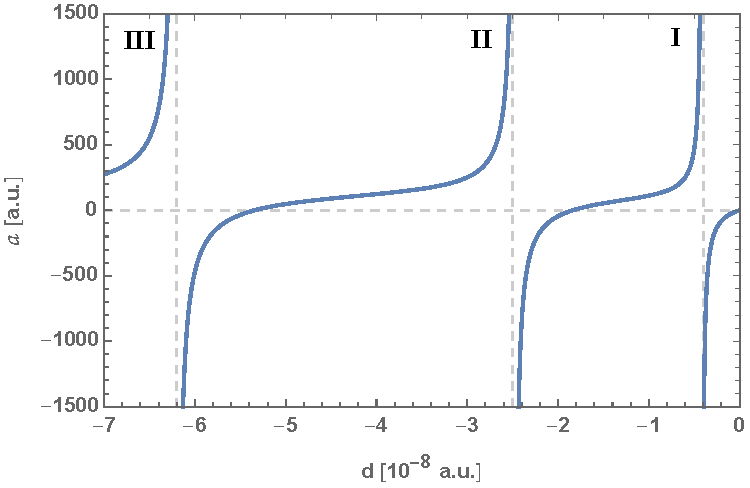
\includegraphics[width=\linewidth]{scatteringlength.pdf}
	\caption{Adiabatic potential curves $U_{\nu}$ as a function of the hyperradius $\rho$ for $a=228 $ .}
	\label{fig:3}
\end{figure}

\begin{figure}
	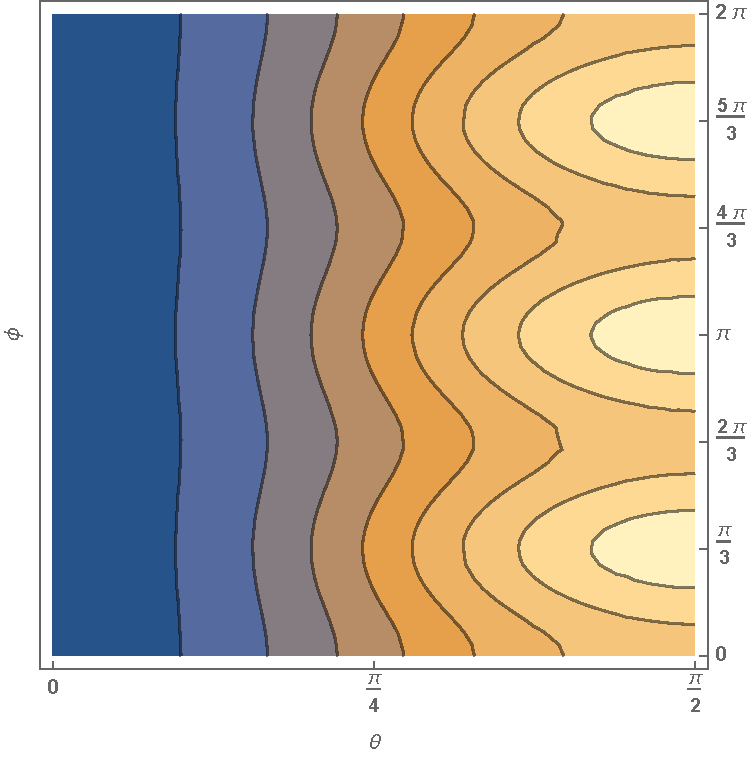
\includegraphics[width=\linewidth]{potential.pdf}
	\caption{Adiabatic potential curves $U_{\nu}$ as a function of the hyperradius $\rho$ for $a=228 $ .}
	\label{fig:3}
\end{figure}

\begin{figure}
	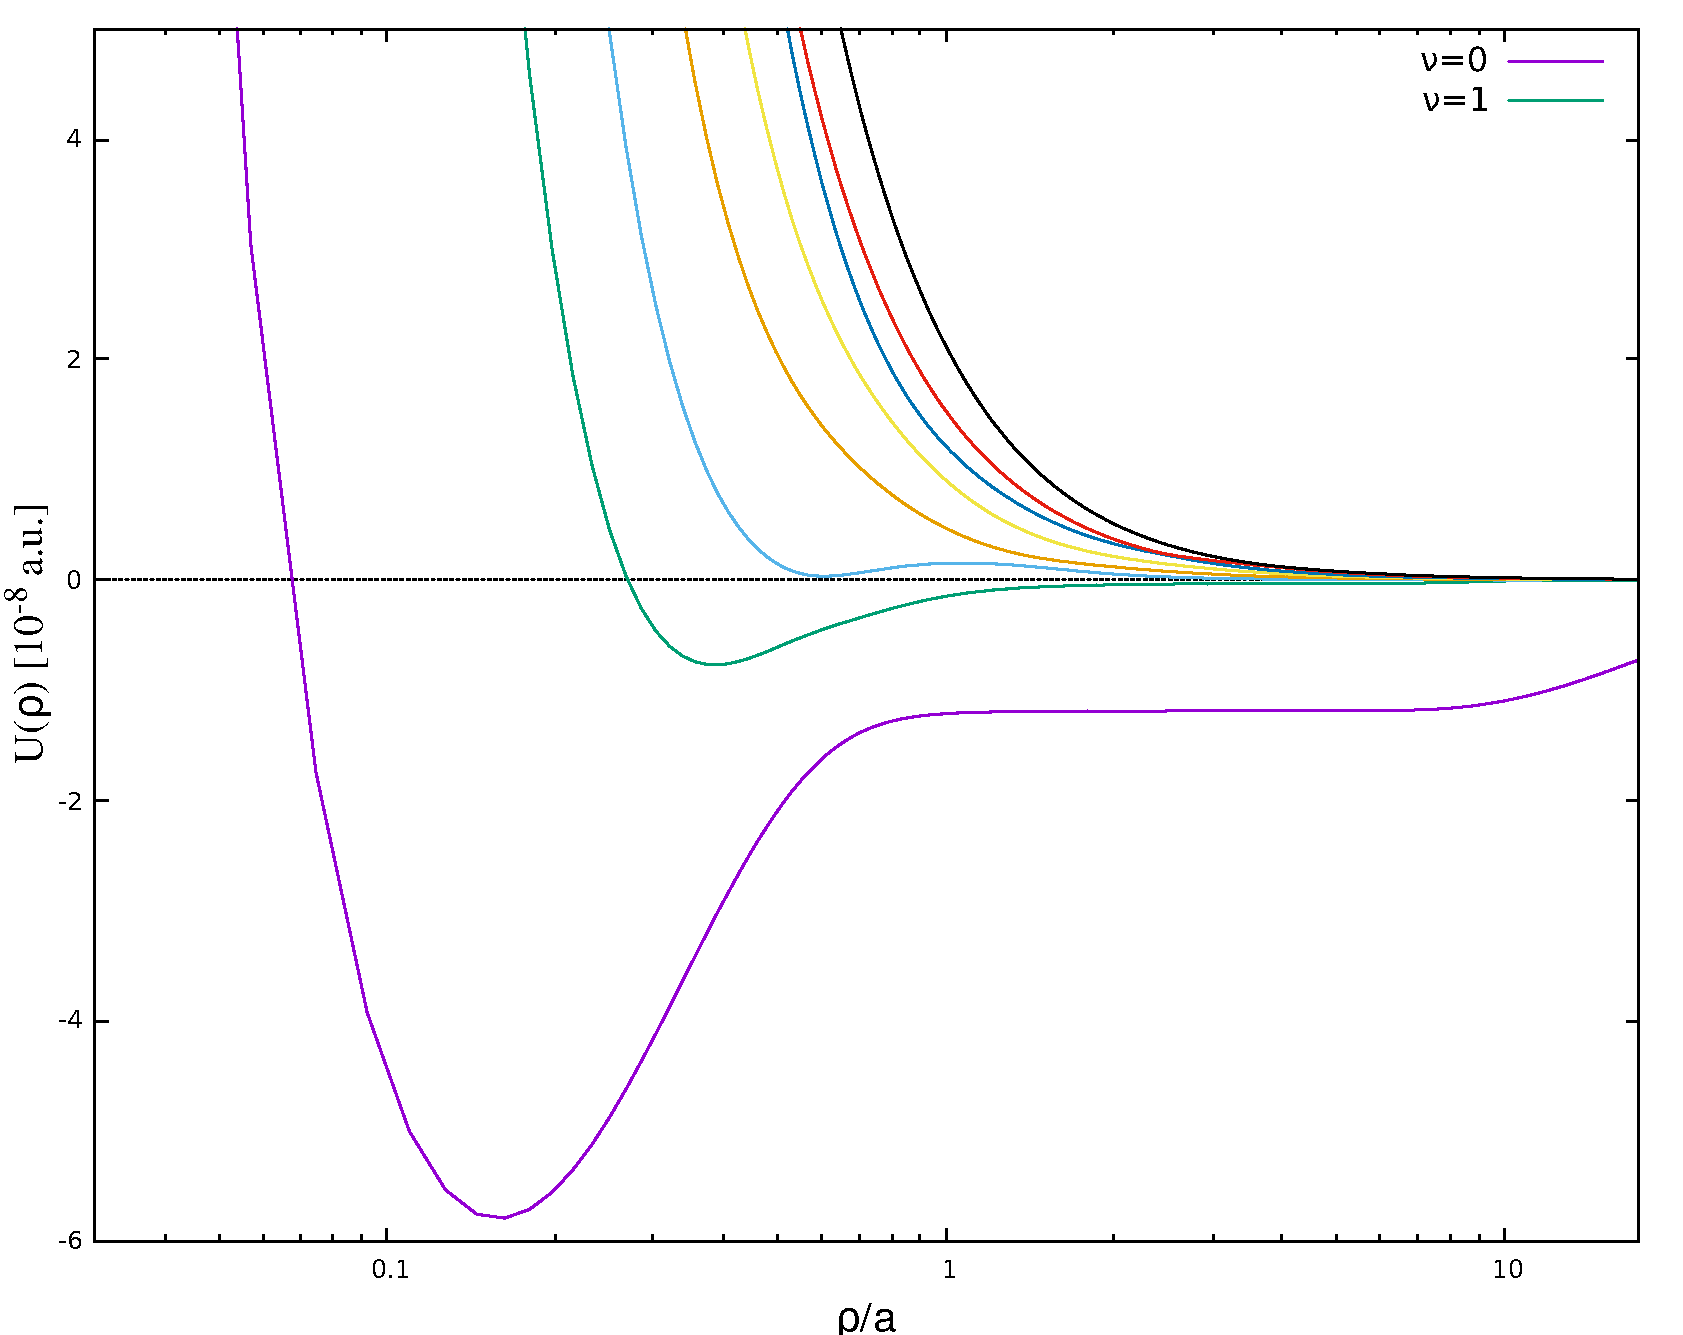
\includegraphics[width=\linewidth]{adiabatic.pdf}
	\caption{Adiabatic potential curves $U_{\nu}$ as a function of the hyperradius $\rho$ for $a=228 $ .}
	\label{fig:3}
\end{figure}

\appendix
\section{Basis splines}\label{B-splines}
A basis spline, or B-spline, of order $k$ is a piecewise polynomial function of degree $(k-1)$ defined on a collection of points, $t_i$, called \textit{knotpoints}. The array formed by these knotpoints are refered to as \textit{knot sequence}, or knot vector, where $t_i\leq t_{i+1}$. B-splines of order $k$ can be defined recursively by the Cox-de Boor formula. With a given knot sequence, the B-splines of order $k=1$ is defined as

\begin{equation}
B_{i,k=1}(x) \doteq
\begin{cases}
1, \quad \text{if} \quad & t_i \leq x < t_{i+1}\\
0,& \text{otherwise} 
\end{cases}
\end{equation}
and if $k>1$

\begin{equation}
B_{i,k}(x) \doteq \frac{x-t_i}{t_{i+k-1}-t_i}B_{i,k-1}(x) + \frac{t_{i+k}-x}{t_{i+k}-t_{i+1}}B_{i+1,k-1}(x).
\end{equation}
The B-splines are local in the sense that they will be non-zero only in a limited region of space. If the numbering is such that the first knot point is $t_1$ and the first  B-spline is $B_{1,k}$, then the B-spline $B_{i,k}$ is non-zero within the region $t_i \leq x \leq t_{i+k}$. On a given knot sequence $(t_1,\ldots , t_N)$ the B-splines form a complete set

\begin{equation}
\sum_{i=1}^{N} B_{i,k}(x_i) = 1.
\end{equation}
By placing $(k-1)$ additional points, called \text{ghost points}, at the endpoints, the B-splines will be confined within the region $t_1 \leq x \leq t_N$, $(k-1)$. This means that $N$ knot points in one dimension correspond to $N-2(k-1)$ physical points in that coordinate dimension. This is a common choice because consequentially, this makes only the first B-spline non-zero at the first physical point. 

\begin{figure}
	\centering  
	\subfigure[$k=1$]{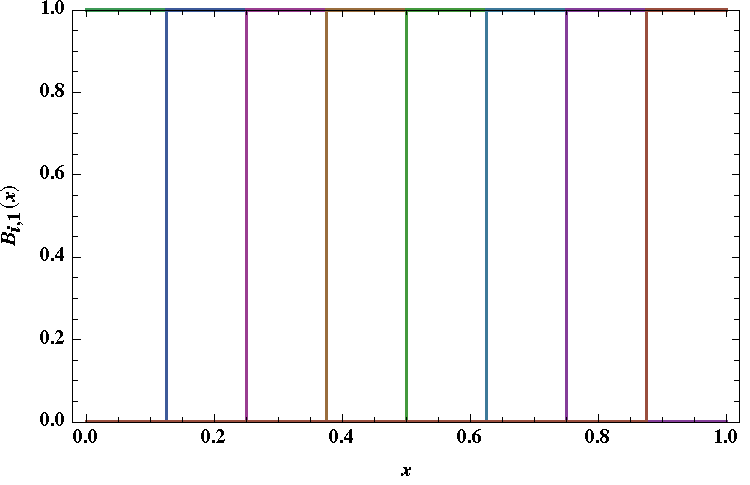
\includegraphics[width=0.45\linewidth]{Bsp1.pdf}}
	\subfigure[$k=2$]{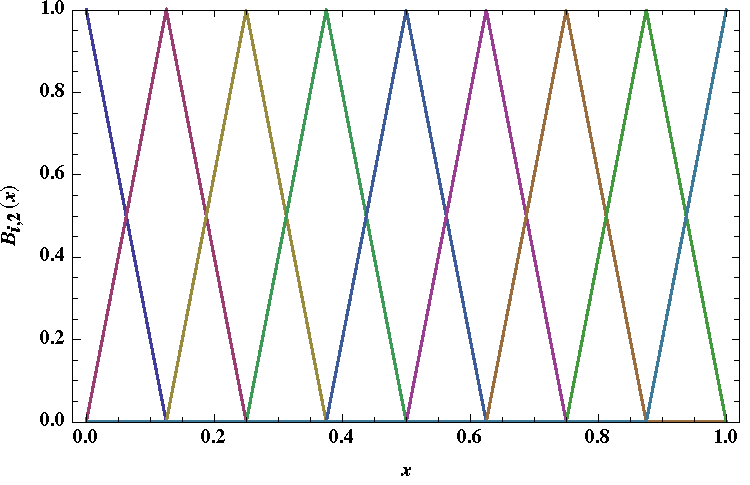
\includegraphics[width=0.45\linewidth]{Bsp2.pdf}}
	\subfigure[ $k=3$]{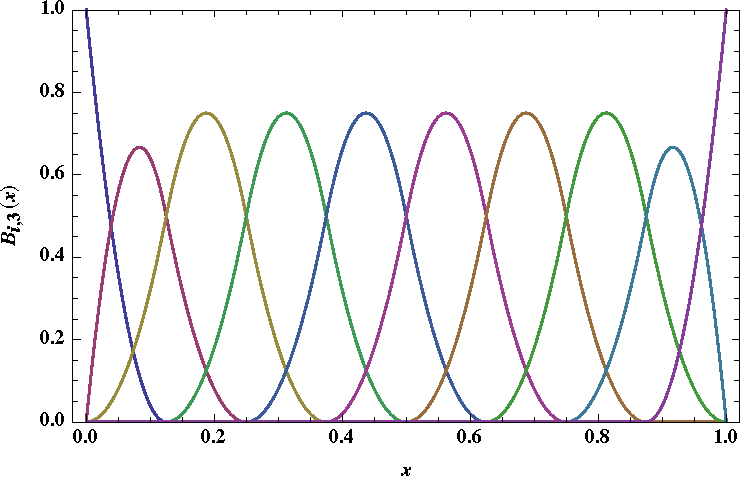
\includegraphics[width=0.45\linewidth]{Bsp3.pdf}}
	\subfigure[ $k=4$]{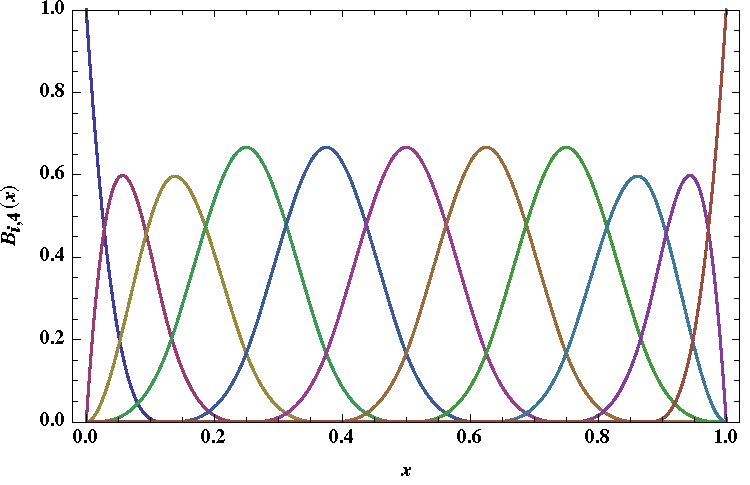
\includegraphics[width=0.45\linewidth]{Bsp4.pdf}}
	\caption{The subfigures above show the B-splines $B_{i,k}(x)$ of different orders $k$ on a one dimensional mesh.}
\end{figure}

The first derivative of a B-spline of order $k$ is given by

\begin{equation}
\frac{\partial}{\partial x}B_{i,k}(x) = (k-1)\bigg(\frac{B_{i,k-1}(x)}{t_{i+k-1}-t_i} + \frac{B_{i+1,k-1}(x)}{t_{i+k}-t_{i+1}}\bigg),
\end{equation}
and the second derivative

\begin{align}
\frac{\partial^2}{\partial x^2}B_{i,k}(x) &= \frac{(k-1)(k-2)B_{i,k-2}(x)}{(t_{i+k-1}-t_i)(t_{i+k-2}-t_i)} - \frac{(k-1)(k-2)B_{i+1,k-2}(x)}{(t_{i+k-1}-t_i)(t_{i+k-1}-t_{i+1})}\nonumber\\
&- \frac{(k-1)(k-2)B_{i+1,k-2}(x)}{(t_{i+k}-t_{i+1})(t_{i+k-1}-t_{i+1})} +  \frac{(k-1)(k-2)B_{i+2,k-2}(x)}{(t_{i+k}-t_{i+1})(t_{i+k}-t_{i+2})}.
\end{align}
B-splines can be used to form basis functions. 

\begin{equation}
f(x_i) = \sum_{n=i-k+1}^{i-1} c_n B_{n,k}(x_i).
\end{equation}

\printbibliography

\end{document}